%==============================================================================
% AES - Symmetrische Verschluesselung in TASM umgesetzt
% Abschlussprojekt "Assemblerprogrammierung" - 19-INB1
%
% Optik nach dem Muster (main.tex) von Tim Kretzschmar.
% Compiler: pdflatex (+ biber fuer das Literaturverzeichnis)
%
%   pdflatex main && biber main && pdflatex main && pdflatex main
%
% Die ehemaligen PDFs liegen als einzelne Dateien in section/ vor und werden
% weiter unten per \input eingeladen. Nicht gewuenschte Teile einfach mit %
% auskommentieren.
%==============================================================================
\documentclass[11pt,a4paper,twoside]{article}
\usepackage[top=1.5in,bottom=1in,left=1.125in,right=1.125in]{geometry}
\usepackage[utf8]{inputenc}
\usepackage{amsmath}
\usepackage{amssymb}
\usepackage[center]{caption}
\usepackage{booktabs}
\usepackage[table,dvipsnames]{xcolor}
\usepackage{color}
\usepackage{float}
\usepackage{needspace}
\usepackage{graphicx}
\usepackage{longtable}
\usepackage{tocloft}
\usepackage{multirow}
\usepackage{multicol}
\usepackage[singlespacing]{setspace}
\usepackage[ngerman]{babel}

% label item in itemize
\usepackage{enumitem}

% Listings (ersetzt minted -> kein -shell-escape noetig)
\usepackage{listings}
\definecolor{LightGray}{gray}{0.95}
\lstdefinelanguage{TASM}{
    morekeywords={MOV,ADD,SUB,XOR,CMP,JMP,JE,JNE,JNC,JC,CALL,RET,PUSH,POP,INT,
        SHL,SHR,ROL,ROR,LOOP,NOP,INC,DEC,PROC,ENDP,ENDS,INCLUDE,DB,DW},
    sensitive=false,
    morecomment=[l]{;},
    morestring=[b]"
}
\lstset{
    language=TASM,
    frame=lines,
    framesep=2mm,
    backgroundcolor=\color{LightGray},
    basicstyle=\ttfamily\footnotesize,
    keywordstyle=\bfseries,
    commentstyle=\itshape\color{gray},
    columns=fullflexible,
    keepspaces=true,
    showstringspaces=false,
    xleftmargin=2mm,
    xrightmargin=2mm,
    aboveskip=3mm,
    belowskip=3mm,
    captionpos=b
}
\renewcommand{\lstlistingname}{Code}
\renewcommand{\lstlistlistingname}{Codeverzeichnis}

% Kopf-/Fusszeile
% https://web.archive.org/web/20220118000906/https://tex.stackexchange.com/questions/109654/page-numbering-different-side-of-heading-for-odd-and-even-page
\usepackage{fancyhdr}
\pagestyle{fancy}
\fancyhf{}
\setlength{\headheight}{14pt}
\fancyhead[C]{
    \ifodd
        \value{page} AES -- Symmetrische Verschlüsselung in TASM
        \small    % Linie weg wenn einkommentiert
    \else
        Abschlussprojekt Assemblerprogrammierung
        \small    % Linie weg wenn einkommentiert
    \fi
}
\fancyhead[R]{\thepage\ifodd\value{page}\else\hfill\fi}

\fancypagestyle{plain}{
}

% url vor biblatex laden (Leerzeichen in \asm{...} erhalten)
\usepackage[obeyspaces]{url}

% Biblatex
\usepackage{csquotes}
\usepackage[
    natbib=true,
    hyperref=true,
    backend=biber,
    style=numeric,
    natbib=true,
    sorting=none,
    defernumbers=true,
    block=nbpar,
    backref=true
]{biblatex}
\addbibresource{bib.bib}
\usepackage{hyperref}

% If you want to break on URL numbers
\setcounter{biburlnumpenalty}{9000}
% If you want to break on URL lower case letters
\setcounter{biburllcpenalty}{9000}
% If you want to break on URL UPPER CASE letters
\setcounter{biburlucpenalty}{9000}

\setlength{\parindent}{0mm} % also nicht vorhanden
\setlength{\parskip}{3mm}
\setlength{\emergencystretch}{2em}

% Grafiken -----------------------------------------------------------------
\usepackage{graphics,graphicx}
\usepackage{calc}
% Abbildungen und Tabellen kapitelweise nummerieren (Abbildung 1.1, 2.1, ...)
\numberwithin{figure}{section}
\numberwithin{table}{section}

% Zeilenabstand ------------------------------------------------------------
\renewcommand{\baselinestretch}{1.25}

% Seitenlayout --------------------------------------------------------------
% twoside setzt \flushbottom: Seiten werden senkrecht auseinandergezogen,
% sobald das naechste Bild nicht mehr passt (grosse Luecken um Ueberschriften).
\raggedbottom
% Gleitobjekte duerfen auf der Seite nach oben/unten wandern statt feststehend
% ([H]) Luecken zu reissen; \floatpagefraction/\textfraction lockern das etwas.
\renewcommand{\topfraction}{0.9}
\renewcommand{\bottomfraction}{0.9}
\renewcommand{\textfraction}{0.1}
\renewcommand{\floatpagefraction}{0.7}

% Inhaltsverzeichnis zentrieren und Tiefe einstellen -----------------------
% per \addto, sonst ueberschreibt babel den Titel beim \begin{document}
\addto\captionsngerman{\renewcommand{\contentsname}{\hfill\bfseries\Large Inhaltsverzeichnis \hfill}}
\renewcommand{\cftaftertoctitle}{\hfill}
\setcounter{secnumdepth}{3}
\setcounter{tocdepth}{3}

% Fußnoten mit kleinen römischen Zahlen
\renewcommand{\thefootnote}{\textcolor{green}{\roman{footnote}}}

% footnote ganz unten auf jeder Seite
\usepackage[bottom]{footmisc}

\usepackage{tabularx}
\usepackage{ltablex}
\usepackage{bm}

\def\Cpp{{C\nolinebreak[4]\hspace{-.05em}\raisebox{.4ex}{\tiny\bf ++}}}

% Variablen ----------------------------------------------------------------
\newcommand{\autorEins}{Tim Michael Kretzschmar}
\newcommand{\autorZwei}{Konstantin Blechschmidt}
\newcommand{\themaProjekt}{AES -- Symmetrische Verschlüsselung in TASM umgesetzt}
% Kürzere Referenzierung
\newcommand{\refPlusName}[1]{\ref{#1} \nameref{#1}}
% Code-Namen (Label, PROC, Variablen, Dateien) in Schreibmaschinenschrift.
% Unterstriche muessen NICHT escaped werden (\asm{Ver_Code.asm}); an ihnen darf
% umgebrochen werden und das Makro ist in \caption{...} verwendbar.
\DeclareUrlCommand\asm{\urlstyle{tt}}
% Haekchen / Kreuz (Testfaelle)
\newcommand{\iconok}{\raisebox{-0.3ex}{
\includegraphics[height=1.1em]{images/icon_ok.png}}}
\newcommand{\iconfehler}{\raisebox{-0.3ex}{
\includegraphics[height=1.1em]{images/icon_fehler.png}}}
% Variablen ----------------------------------------------------------------

% Eigenschaften einstellen
\hypersetup{
    pdftitle={\themaProjekt},
    pdfauthor={\autorEins, \autorZwei},
    pdfcreator={\autorEins, \autorZwei},
    pdfkeywords={AES} {TASM} {Assembler},
    pdfnewwindow = true,
    colorlinks,
    pdfstartview = FitH,
    bookmarksopen = true,
    bookmarksnumbered = true,
    linkcolor = black,
    urlcolor = blue,
    plainpages = false,
    hypertexnames = false,
    citecolor = blue
}

% Dokument -----------------------------------------------------------------
\begin{document}
    % Deckblatt (ehemals Titelseite der AES.pdf)
    % Deckblatt (ehemals Titelseite der AES.pdf)
\thispagestyle{empty}
\begin{center}
    \vspace*{0.5cm}
    {\bfseries\Huge AES}\\[1mm]
    {\bfseries\Large --}\\[6mm]
    {\bfseries\Large Symmetrische Verschlüsselung in TASM umgesetzt}\\[4mm]
    {\large Dokumentation zur Version \versionProjekt}\\[1.2cm]
    {\large erstellt von}\\[8mm]
    {\bfseries\Large \autorEins}\\[1mm]
    {\bfseries\Large \autorZwei}\\[1.5cm]
    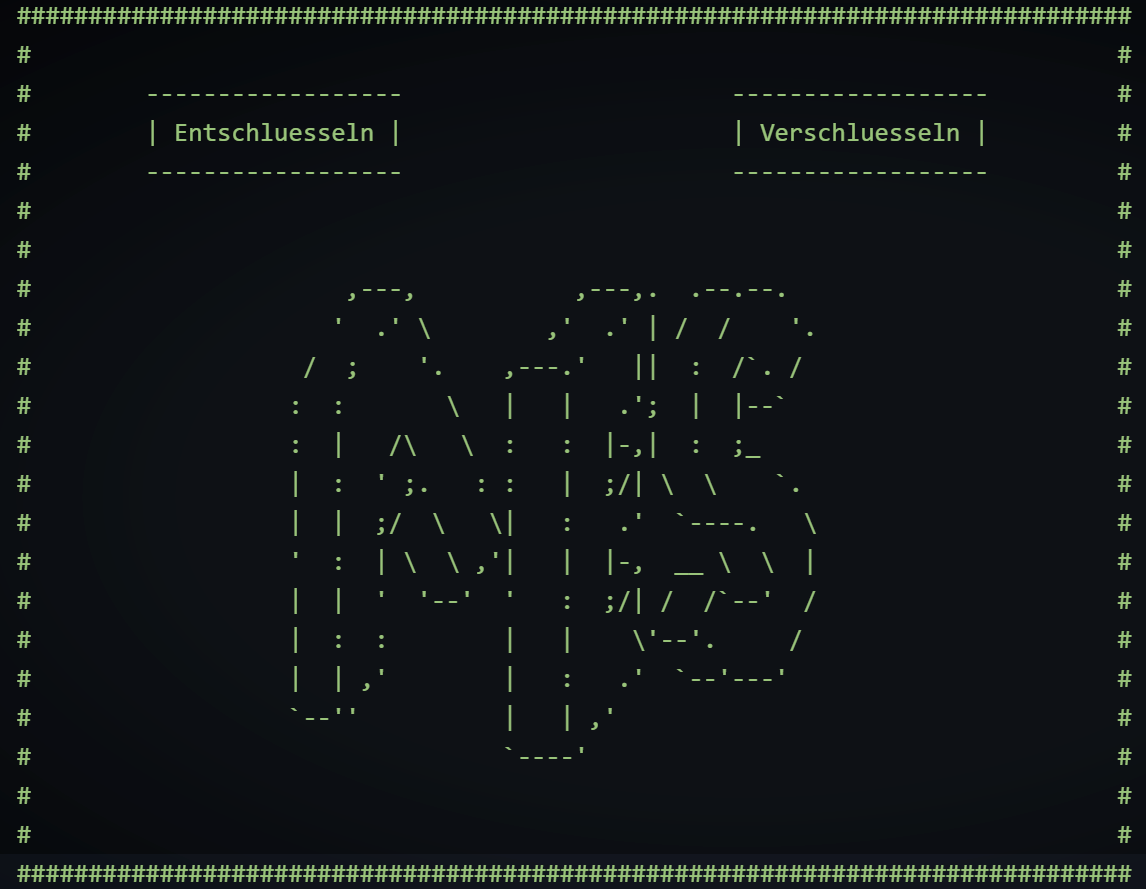
\includegraphics[width=.85\textwidth]{images/cover_dosbox.png}\\[1.5cm]
    {\bfseries Abschlussprojekt \glqq Assemblerprogrammierung\grqq{} -- 19-INB1}
\end{center}
\newpage


    % Inhaltsverzeichnis
    \phantomsection
    \addcontentsline{toc}{section}{Inhaltsverzeichnis}
    \tableofcontents\label{Inhaltsverzeichnis}

    % ---- Handbuch (ehemals AES.pdf, Kapitel 1 bis 3) ----
    \newpage
    % Kapitel 1 -- Einleitung (Stand: Version 2.0.0)
\section{Einleitung}\label{sec:einleitung}
AES wurde von Joan Daemen und Vincent Rijmen (unter dem Alias Rijndael) entwickelt und ist als Advanced Encryption Standard in \cite{fips197} festgeschrieben. Es basiert auf dem Prinzip der symmetrischen Verschlüsselung, bei der derselbe Schlüssel zum Ver- und zum Entschlüsseln dient, und gilt mit seinen verschiedenen Standards als eines der besten Verschlüsselungsverfahren der Welt. Dies ist bedingt durch die Tatsache, dass bis heute kein effektiver Algorithmus gefunden wurde, welcher die Brute-Force-Methode zum Entschlüsseln des Chiffretextes umgeht. Da in absehbarer Zeit die Prozessorleistung keinen sonderlichen Leistungsschub mehr erhalten wird, ist die Schlüssellänge für die Sicherheit ausschlaggebend; also die Dauer der Entschlüsselung.

\subsection{Was dieses Programm umsetzt}
Die hier als Assemblerprogramm (TASM, Prozessor \asm{.486}, Ausführung in der DOS-Box) umgesetzte Variante beruht auf dem Grundgedanken von AES, \emph{ist aber nicht AES nach \cite{fips197}}. Sie arbeitet nicht mit einem einzelnen 16-Byte-Block, sondern mit einem \emph{Zustand} aus 64 Bytes, der in vier unabhängige $4\times4$-Blöcke gegliedert ist (Abschnitt~\ref{sec:zustand}). Der Schlüssel hat ebenfalls 64 Bytes à 8~Bit (also je Stelle 256 mögliche Werte, $0\ldots255$, was der erweiterten ASCII-Tabelle entspricht). Tabelle~\ref{tab:vergleich} stellt den Standard der umgesetzten Variante gegenüber.

\begin{table}[!htbp]
    \centering
    \small
    \renewcommand{\arraystretch}{1.15}
    \caption{AES nach FIPS-197 im Vergleich zur Umsetzung in Version \versionProjekt}\label{tab:vergleich}
    \begin{tabular}{@{}p{3.2cm}p{4.9cm}p{5.4cm}@{}}
        \toprule
        & \textbf{AES (FIPS-197)} & \textbf{diese Umsetzung} \\
        \midrule
        Blockgröße & 16 Byte (ein $4\times4$-Block) & 64 Byte, als vier unabhängige $4\times4$-Blöcke \\
        Schlüssellänge & 128, 192 oder 256 Bit & 64 Byte (512 Bit); Standardschlüssel eingebaut, eigener Schlüssel eingebbar \\
        Rundenzahl & 10, 12 oder 14 & 2 Runden mit abschließender S-Box-Stufe (aktiver Ablauf) \\
        SubBytes & S-Box & identisch (AES-S-Box, 256 Einträge) \\
        ShiftRows & Zeile $r$ um $r$ Stellen nach links & identisch, je Block \\
        MixColumns & in jeder Runde außer der letzten & als \asm{ShiftColumn} und \asm{ShiftColumn_1} vorhanden, im aktiven Ablauf \emph{nicht} aufgerufen \\
        Schlüsselexpansion & wortweise, \asm{RotWord}/\asm{SubWord}, \asm{Rcon} & eigenes Verfahren: Byte-Präfix-XOR mit S-Box-Wert und rotierender Konstante (\asm{5Fh}) \\
        \bottomrule
    \end{tabular}
\end{table}

Daraus folgt: Das Verfahren ist \emph{AES-ähnlich} und \textbf{nicht für den Schutz echter Daten geeignet}. Ohne MixColumns im aktiven Ablauf gibt es keine Diffusion; ein Klartextbyte beeinflusst genau ein Chiffrebyte (Kapitel~\ref{sec:einschraenkungen}). Der Zweck des Projekts ist, die Bausteine von AES in Assembler nachzuvollziehen und im Detail zu verstehen.

Die folgenden Schemata zeigen den \emph{AES-Standardablauf} als Vorbild. Welche Schritte das Programm tatsächlich in welcher Reihenfolge ausführt, steht in Kapitel~\ref{sec:ablauf-beispiel} und in den Abschnitt~\ref{sec:ablauf-v} und~\ref{sec:ablauf-e}.

\begin{figure}[!htbp]
    \centering
    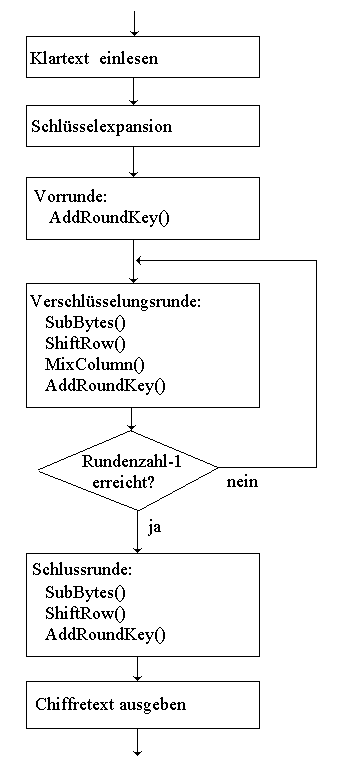
\includegraphics[height=0.5\textheight,keepaspectratio]{images/schema_verschluesselung.png}
    \caption{Schema Verschlüsselung mit AES (Standardablauf) -- Quelle: \cite{ceilers_ver}}
    \label{fig:schema-ver-1}
\end{figure}

\begin{figure}[!htbp]
    \centering
    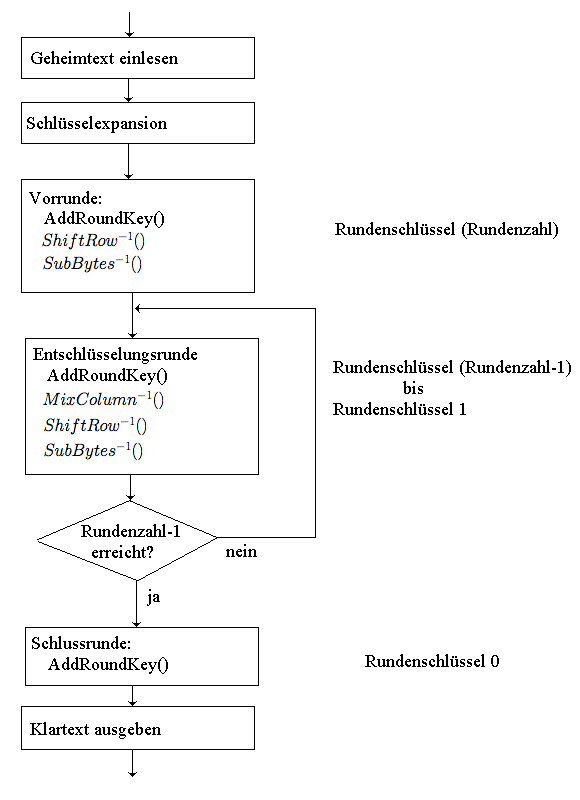
\includegraphics[height=0.5\textheight,keepaspectratio]{images/schema_entschluesselung.png}
    % Im PDF stand hier faelschlich ebenfalls "Verschluesselung".
    \caption{Schema Entschlüsselung mit AES (Standardablauf) -- Quelle: \cite{ceilers_ent}}
    \label{fig:schema-ent-1}
\end{figure}

\subsection{Versionen}
Dieses Dokument beschreibt die \textbf{Version \versionProjekt} (Branch \texttt{v2.0.0}). Die ursprüngliche Abgabe aus dem Jahr 2021 ist die \emph{Version 1.0} (Stand im Git: Commit \commit{89f8212}). Sie wurde damals in fünf getrennten PDF-Dokumenten beschrieben; diese Beschreibungen sind in dieses Dokument eingearbeitet und auf den Stand~\versionProjekt\ gebracht worden. Was sich gegenüber Version~1.0 geändert hat, steht gesammelt in Kapitel~\ref{sec:aenderungen}; die zugehörige Erklärung der Autoren in Kapitel~\ref{sec:erklaerung}.

\subsection{Aufbau dieses Dokuments}
\begin{description}[leftmargin=!,labelwidth=3.4cm,noitemsep]
    \item[Kapitel~\ref{sec:grundlagen}] Datenmodell, Rechnen in $\mathrm{GF}(2^8)$, Registerrollen und Bildschirmadressen -- die Grundlagen, die alle weiteren Kapitel voraussetzen.
    \item[Kapitel~\ref{sec:asm-dateien}] Jede ASM-Datei, jede \asm{PROC} und jedes wichtige Label, mit Registern und Befehlen.
    \item[Kapitel~\ref{sec:ablauf-beispiel}] Ein durchgehendes Zahlenbeispiel (Klartext \glqq Hallo\grqq) durch alle Schritte.
    \item[Kapitel~\ref{sec:batch}--\ref{sec:einschraenkungen}] Batch-Dateien, Bedienung, Funktionsumfang und bekannte Einschränkungen.
    \item[Kapitel~\ref{sec:aenderungen}--\ref{sec:tests}] Änderungen in Version~\versionProjekt, Entwurfsskizze und Tests.
    \item[Kapitel~\ref{sec:erklaerung}] Erklärung der Autoren.
\end{description}

    \newpage
    % Ehemals AES.pdf, Kapitel 2
% Hinweis: Stellen, die durch Version 2.0.0 (S-Box-Korrektur, ShiftRow,
% eigener Schluessel, MixColumns + Inverse) inhaltlich ueberholt sind, sind mit
% "% TODO v2.0.0" markiert. Der Text entspricht sonst dem urspruenglichen PDF.
\section{Die ASM-Dateien und ihr Inhalt}\label{sec:asm-dateien}

\textbf{HINWEIS:} Zu jeder Datei findet hier eine kurze Beschreibung statt. Meist ist jedoch die genauere Erklärung im Quelltext als Kommentar hinter den jeweiligen Befehlszeilen zu finden. Zusätzlich gibt es im Kopf jeder Datei eine Beschreibung, die diesem Werk ähnelt. Es soll lediglich dazu dienen, diese Kopf-Kommentare zu erweitern, noch besser zu strukturieren und einen allgemeinen Überblick zu erhalten.

%------------------------------------------------------------------------------
\subsection{Grafische Übersicht über alle ASM-Dateien}
Hier sind alle ASM-Dateien aufgeführt. Gleichzeitig soll das Zusammenspiel der \asm{AES.asm}, der \asm{VER_Code.asm} und \asm{ENT_Code.asm}, sowie den \asm{Ablauf_V.asm} und \asm{Ablauf_E.asm} graphisch demonstriert werden, was im späteren Verlauf schriftlich erklärt wird.

\begin{figure}[!htbp]
    \centering
    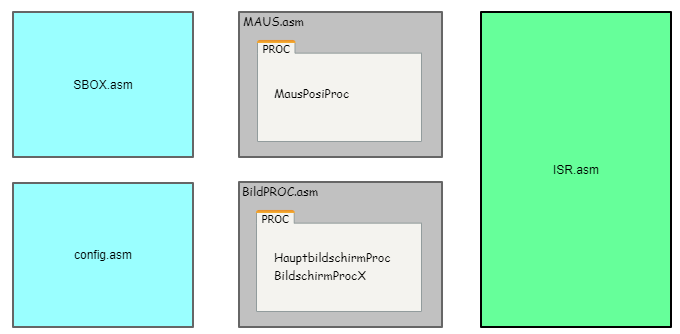
\includegraphics[width=0.8\textwidth]{images/uebersicht_dateien.png}
    \caption{Übersicht über die ASM-Dateien (SBOX, config, MAUS, BildPROC, ISR)}
    \label{fig:uebersicht-dateien}
\end{figure}

\begin{figure}[!htbp]
    \centering
    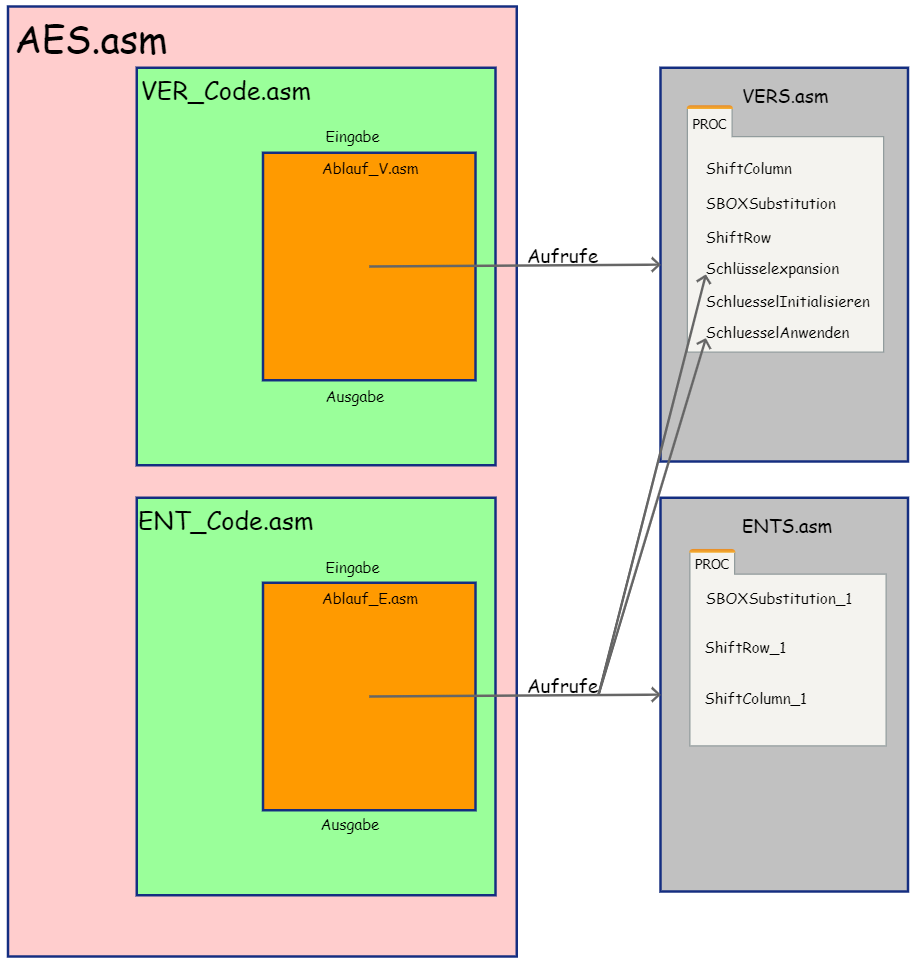
\includegraphics[height=0.55\textheight,keepaspectratio]{images/uebersicht_zusammenspiel.png}
    \caption{Zusammenspiel von AES.asm, VER\_Code.asm, ENT\_Code.asm, VERS.asm und ENTS.asm}
    \label{fig:uebersicht-zusammenspiel}
\end{figure}

%------------------------------------------------------------------------------
\subsection{AES.asm}
Hier findet die grundlegende Verwaltung des Ablaufes statt. Diese Datei kann man auch als \asm{main} bezeichnen. Im Folgenden wird auf die einzelnen Label und ihre Funktionalitäten näher eingegangen.

\subsubsection{Beginn (Label)}
Laden des Data-Segmentes in \asm{DS}. Im Data-Segment sind 2 \asm{INCLUDE}s vorhanden:
\begin{enumerate}[label=\arabic*,noitemsep]
    \item \asm{SBOX.asm}
    \item \asm{config.asm}
\end{enumerate}

\subsubsection{Hauptbildschirm darstellen (Label)}
Wie der Name schon erwarten lässt, wird hier der Hauptbildschirm gezeichnet. Dies geschieht über den Aufruf einer \asm{PROC} \asm{HauptbildschirmProc}. Davor wird jedoch ebenfalls noch in diesem Label die Maus-Klick-Funktion belegt. Dies geschieht durch das Freisetzen der beiden Primärmaustasten links und rechts, sowie dem Definieren des \asm{OFFSET}s der \asm{PROC} \asm{MausPosiProc}.

\subsubsection{Endlosschleife (Label)}
In der Endlosschleife wird auf einen Tastaturdruck gewartet (\asm{INT 16h}, Unterfunktion \asm{1h}). Nachdem dieser erfolgt ist, folgt ein \asm{CMP} mit dem Ziel, die ESC-Taste zu detektieren. Bei einer Übereinstimmung springt das Programm zu dem \asm{ESCEnde} (Label). Andernfalls wird eine Überprüfung des Inhalts der Variable \asm{bool_Ent_Ver} vorgenommen. Hier können 3 Fälle eintreten.

\begin{center}
    \begin{tabular}{@{}lll@{}}
        Wert = 1 & Springe zum & \asm{EntschluesselungBeginn} (Label) \\
        Wert = 2 & Springe zum & \asm{VerschluesselungBeginn} (Label) \\
        Wert = 3 & Springe zurück zur & \asm{Endlosschleife} (Label) \\
    \end{tabular}
\end{center}

\subsubsection{VerschluesselungBeginn (Label)}
Hier wird über ein \asm{INCLUDE} der Code für das Verschlüsseln aus der \asm{Ver_Code.asm} eingefügt und durchlaufen. Nach dessen Abschluss wird die Variable \asm{bool_Ent_Ver} wieder auf 3 gesetzt, also in den Wartezustand überführt. Als letzte Handlung folgt ein \asm{JMP} zum \asm{HauptbildschirmDarstellen} (Label).

\subsubsection{EntschluesselungBeginn (Label)}
Hier wird über ein \asm{INCLUDE} der Code für das Entschlüsseln aus der \asm{Ent_Code.asm} eingefügt und durchlaufen. Nach dessen Abschluss wird die Variable \asm{bool_Ent_Ver} wieder auf 3 gesetzt, also in den Wartezustand überführt. Als letzte Handlung folgt hier ebenfalls ein \asm{JMP} zum \asm{HauptbildschirmDarstellen} (Label).

\subsubsection{ESCEnde (Label)}
In diesem Programmteil wird eine Überprüfung der Variable \asm{bool_Ent_Ver} auf den Wert 3 vorgenommen. Sollte eine Übereinstimmung vorliegen, so wird der Sprung (\asm{JMP}) zum \asm{Ende} (Label) vorgenommen, andernfalls springt das Programm zum \asm{HauptbildschirmDarstellen} (Label). Somit wird ein ungewolltes Verlassen aus dem Ent- bzw. Verschlüsselungsbildschirm verhindert.

\subsubsection{Ende (Label)}
Als Erstes wird der Bildschirm geleert. Dies geschieht über den erneuten Aufruf des Videomodus 3, ohne jedoch etwas Weiteres darzustellen. Anschließend erfolgen die zwei Standardzeilen in TASM für das Zurückkehren in die DOS-Box:

\begin{lstlisting}[language=TASM]
MOV AH, 4Ch
INT 21h
\end{lstlisting}

%------------------------------------------------------------------------------
\subsection{MAUS.asm}
\subsubsection{MausPosiProc (PROC)}
In dieser \asm{PROC} wird überprüft, wo sich der Mauszeiger beim Klicken befand. Je nach Ergebnis wird dann ein anderer Bildschirm angezeigt. Dabei gibt es drei Fälle:

\begin{enumerate}[label=\arabic*,noitemsep]
    \item Keine Schaltfläche getroffen
    \item Entschlüsseln getroffen
    \item Verschlüsseln getroffen
\end{enumerate}

Der simpelste Fall ist die Nummer 1. Hier wird einfach nichts getan, außer den Zustandsspeicher \asm{bool_Ent_Ver} auf 3 zu setzen, was als \glqq nichts zu tun\grqq{} interpretiert wird. Fall 2 setzt diese Variable jedoch auf 1 (entspricht Entschlüsselung) und zeichnet anschließend den \asm{Hauptbildschirm2}. Dieser beinhaltet die Flächen für die Text- und Schlüsseleingabe. Sollte jedoch kein oder ein nur unvollständiger Schlüssel eingegeben werden, so wird automatisch der vordefinierte Schlüssel aus der \asm{config.asm} für den weiteren Ablauf verwendet.

Auf der folgenden Seite ist der Ablauf der Feststellung, ob und welche Schaltfläche getroffen wurde, graphisch dargestellt.

\begin{figure}[!htbp]
    \centering
    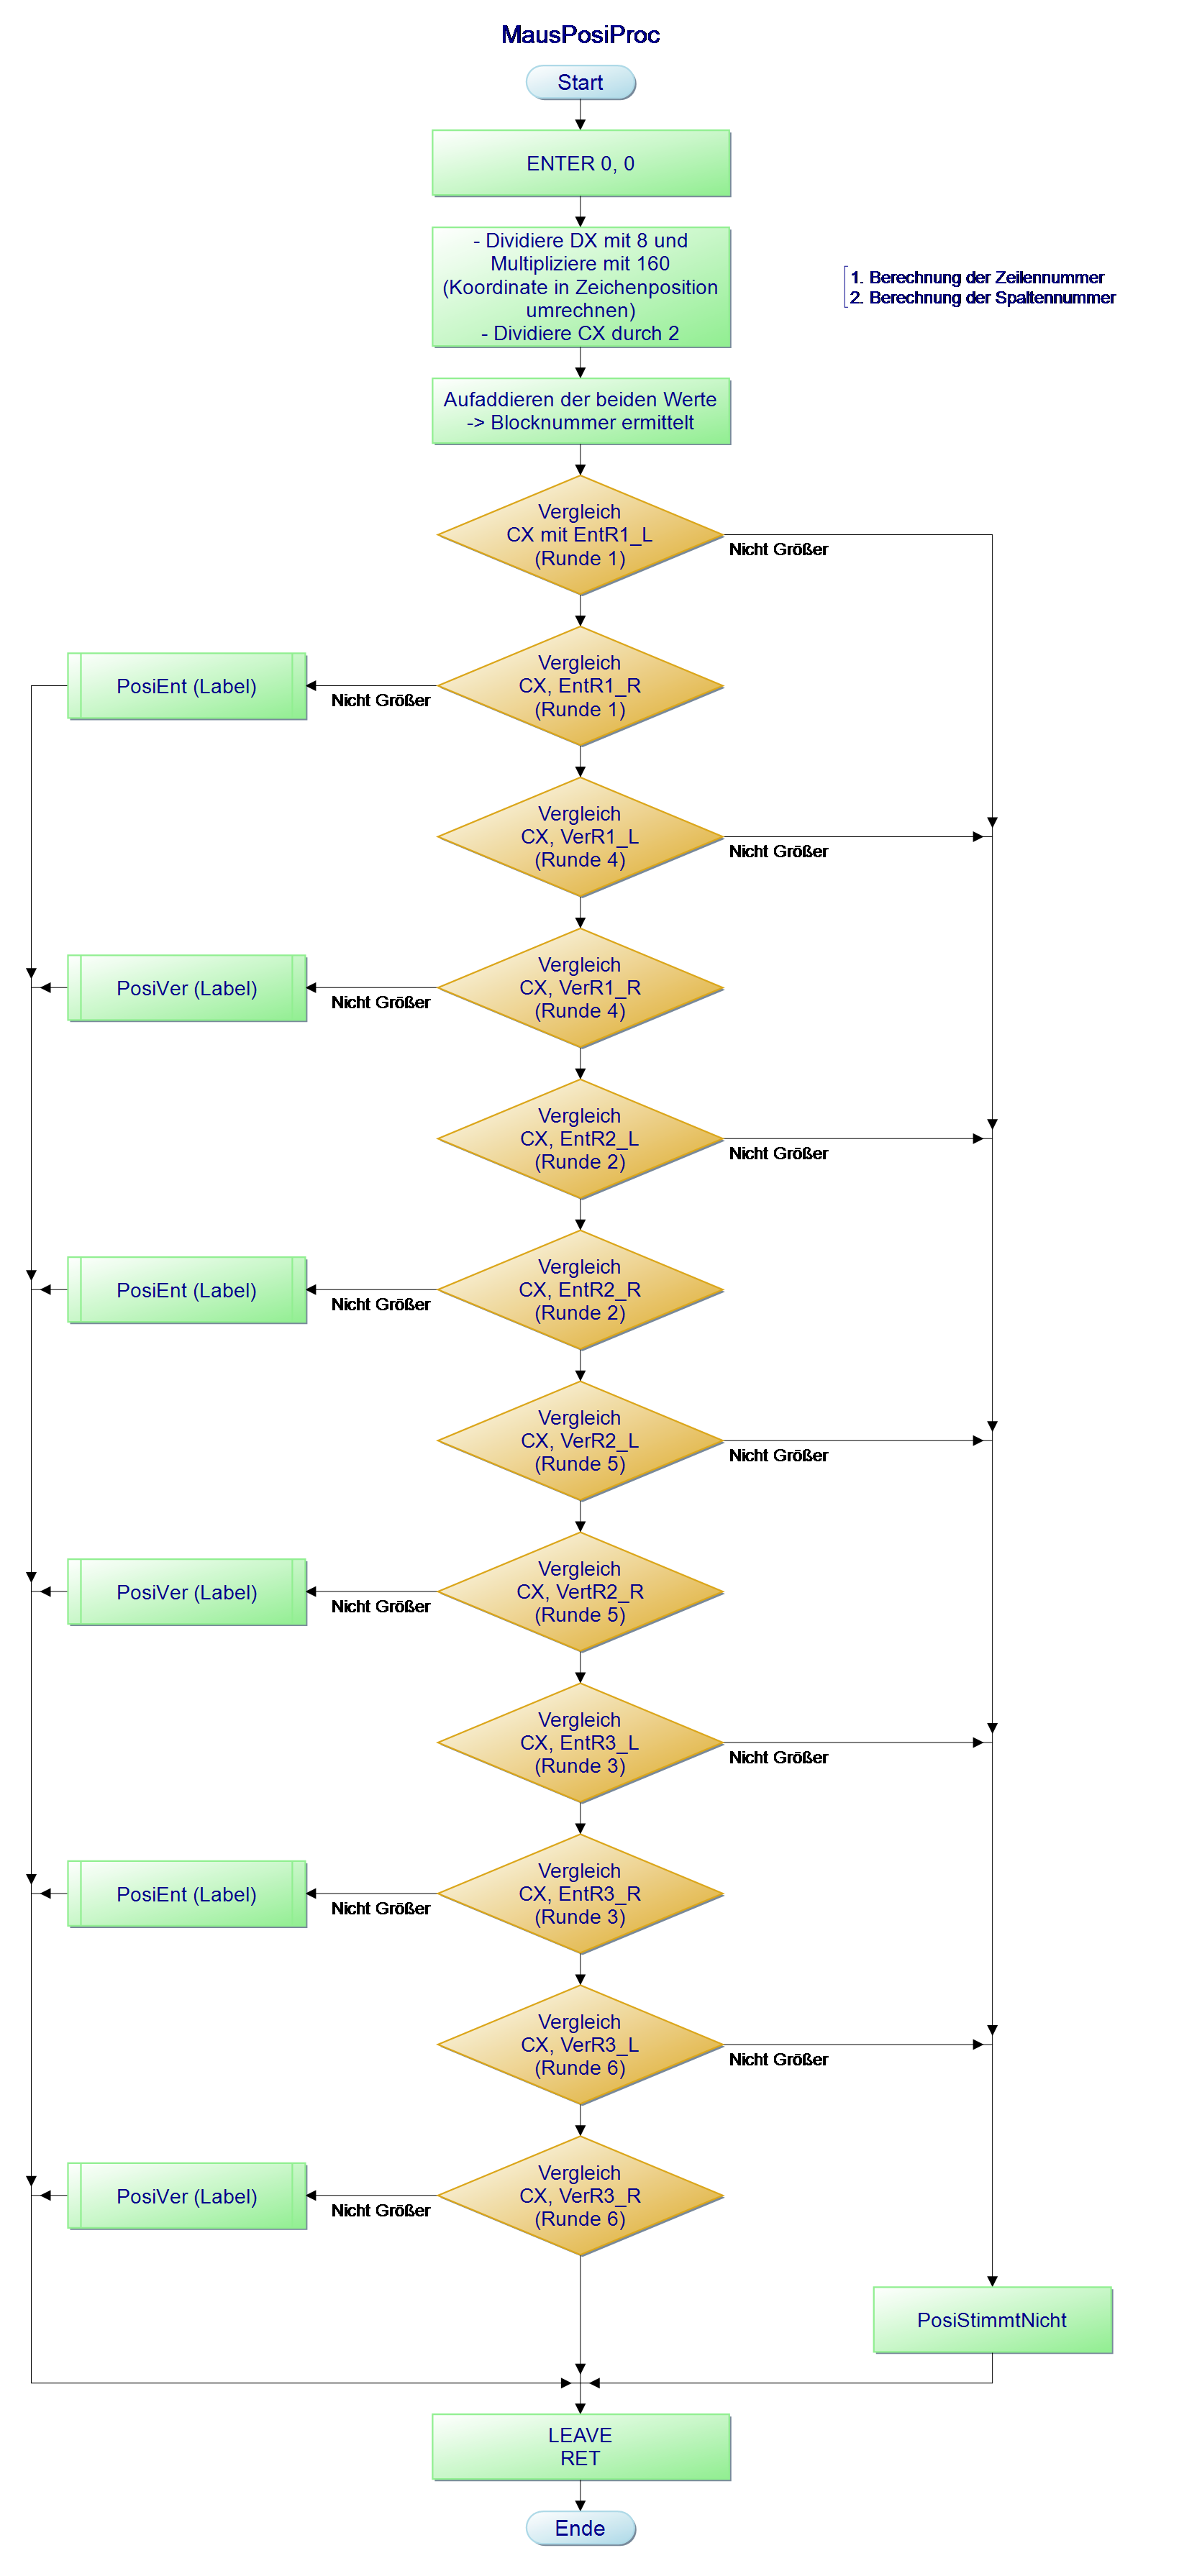
\includegraphics[height=0.8\textheight,keepaspectratio]{images/pap_mausposiproc.png}
    \caption{Programmablaufplan der \texttt{MausPosiProc}}
    \label{fig:pap-mausposiproc}
\end{figure}

%------------------------------------------------------------------------------
\subsection{Ver\_Code.asm}
Nachdem der Bildschirm zum Verschlüsseln aufgerufen wurde, ist hier der Ablauf von Klartext-Eingabe, Schlüssel in Hex-Werten und chiffrierter Textausgabe (ebenfalls in Hex-Werten) definiert. Die Klartextlänge ist auf 64 Zeichen und die Schlüssellänge auf 128 Zeichen beschränkt. 2 Eingaben beim Schlüssel erzeugen einen internen Hex-Wert.

Durch einen \asm{INCLUDE} von der \asm{Ablauf_V.asm}, in der die Struktur der Verschlüsselung beschrieben ist, wird in diesem Programmteil die interne Verschlüsselung an sich aufgerufen.

%------------------------------------------------------------------------------
\subsection{Ent\_Code.asm}
Nachdem der Bildschirm zum Entschlüsseln über die dafür existierende \asm{PROC} (siehe Absatz~\ref{sec:bildschirmprocx} \nameref{sec:bildschirmprocx}) gezeichnet wurde, kommt es hier ebenfalls zu einer Eingabe. Dieses Mal erfolgt die Texteingabe wegen des zu entschlüsselnden Zeichensatzes über hexadezimale Werte. Erlaubt sind dabei 0 bis 9 und A bis F. Nur Großbuchstaben werden akzeptiert.

Nach dem selben Muster erfolgt auch die Eingabe für den Schlüssel. Die Schlüsseleingabe wird den Standardschlüssel (welcher fest integriert ist) soweit überschreiben, wie diese Eingabe erfolgt. Es können wieder maximal 128 Zeichen eingegeben werden. 2 Eingaben erzeugen einen internen Hex-Wert.

Vor der Ausgabe des Klartextes wird in diesem Programmabschnitt ähnlich der \asm{Ver_Code.asm} ein \asm{INCLUDE} durchgeführt, welcher den Ablauf der Entschlüsselung aus der \asm{Ablauf_E.asm} aufruft.

%------------------------------------------------------------------------------
\subsection{Ablauf\_V.asm}
In dieser ASM-Datei wird der allgemeine Ablauf geregelt, der bei einer Verschlüsselung stattfindet. Die Umsetzung in den Labels erfolgte nach diesem Muster (siehe nächste Seite), welches nochmal textuell ergänzend erklärt ist.

\begin{figure}[!htbp]
    \centering
    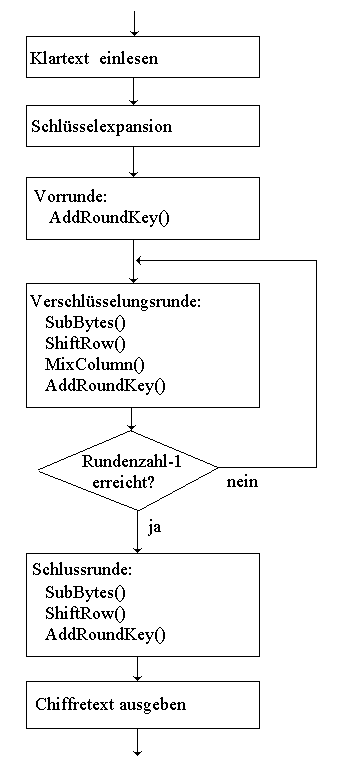
\includegraphics[height=0.5\textheight,keepaspectratio]{images/schema_verschluesselung.png}
    \caption{Schema Verschlüsselung mit AES -- Quelle: \cite{ceilers_ver}}
    \label{fig:schema-ver-2}
\end{figure}

\subsubsection{AblaufVerVorrunde (Label)}
Hier geschieht lediglich die Verrechnung mit dem Rundenschlüssel nach der ersten Schlüsselexpansion.

\subsubsection{AblaufVer (Label)}
Dies sind die Hauptrunden der Verschlüsselung. Die Anzahl der Runden werden in der \asm{Rundenanzahl} definiert. Durch den Beginn des Vergleichswertes in \asm{CL} (Register) mit 1 wird auch tatsächlich die Anzahl der gewünschten Runden durchlaufen. Die Schlussrunde läuft anders ab, wird aber als (1) Runde mitgezählt.

In der Reihenfolge werden hier die einzelnen Werte erst substituiert (Prinzip siehe \asm{SBOX.asm}), dann die Reihen rotiert (\asm{ShiftRow}) mit anschließendem \asm{ShiftColumn}. Zuletzt findet eine Schlüsselexpansion statt, damit der Rundenschlüssel erzeugt und nachfolgend auf den \asm{TastaturBuffer} gerechnet wird.

\subsubsection{AblaufVerEndrunde (Label)}
Diese letzte Runde findet ähnlich den Hauptrunden statt, jedoch wird hier die Verrechnung der Spalten per \asm{ShiftColumn} weggelassen. Die nun erwähnte Ausgabe wird wiederum in der \asm{Ver_Code.asm} geregelt.

%------------------------------------------------------------------------------
\subsection{Ablauf\_E.asm}
In dieser ASM-Datei wird der allgemeine Ablauf geregelt, der bei einer Entschlüsselung stattfindet. Die Umsetzung in den Labels erfolgte nach dem Muster auf der nächsten Seite, welches nochmal textuell ergänzend erläutert ist. AES ist ein symmetrisches Verfahren. Somit ist erkennbar, dass die Entschlüsselung wie die inverse Verschlüsselung stattfindet.

\begin{figure}[!htbp]
    \centering
    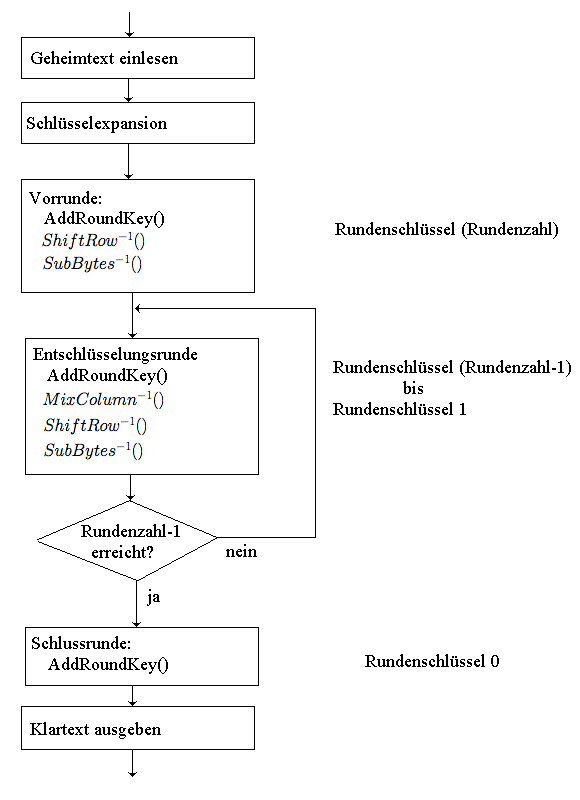
\includegraphics[height=0.5\textheight,keepaspectratio]{images/schema_entschluesselung.png}
    \caption{Schema Entschlüsselung mit AES -- Quelle: \cite{ceilers_ent}}
    \label{fig:schema-ent-2}
\end{figure}

\subsubsection{AblaufEntVorrunde (Label)}
In dieser Vorrunde findet nach Schlüsselexpansion die Verrechnung mit diesem Rundenschlüssel, dann ein inverser \asm{ShiftRow} (siehe \asm{ShiftRow_1}) und schließlich die inverse Substitution mit der invertierten \asm{SBOX} statt.

\subsubsection{AblaufEnt (Label)}
Hier findet solange die Hauptrunde der Entschlüsselung statt, wie der Rundzähler aus \asm{CL} nicht gleich der Rundenanzahl ist. Damit ist gemeint, dass zunächst der Rundenschlüssel expandiert und aufgerechnet wird, dann die inverse Spaltenrechnung stattfindet, anschließend die inverse Zeilenmischung sowie die abschließende Substitution mit der inversen \asm{SBOX}.

\subsubsection{AblaufEntEndrunde (Label)}
In dieser Schlussrunde wird, dank dem symmetrischen Verfahren, lediglich der Rundenschlüssel auf den \asm{TastaturBuffer} gerechnet. Dies entspricht der Vorrunde des Verschlüsselungsablaufes.

%------------------------------------------------------------------------------
\subsection{VERS.asm}
\subsubsection{SchluesselInitialisieren (PROC)}
Die Funktion dieser \asm{PROC} ist einfach, da der gesamte, fest in der \asm{config.asm} implementierte, Standardschlüssel in den \asm{Rundenschluessel_Expand} kopiert wird. Somit bleibt der \asm{Rundenschluessel_Expand} bei einer nicht erfolgten Eingabe durch den Benutzer nicht leer. Ebenfalls wird die Rundenkonstante initialisiert mit dem Wert $5F_{\text{hex}}$.

\textbf{HINWEIS:} Bei der manuellen Eingabe eines Schlüssels oder Teilschlüssels, wird der jeweilige Bereich, wie weit die Eingabe reicht, überschrieben und somit der Benutzerwunschschlüssel verwendet.

\subsubsection{SchluesselAnwenden (PROC)}
Mit dieser \asm{PROC} wird das Anwenden des Rundenschlüssels auf das Array im \asm{TastaturBuffer} beschrieben.

\subsubsection{Schluesselexpansion (PROC)}
Die Rundenschlüsselexpansion findet nach folgendem Muster statt:

\begin{align*}
    k_{\text{Runde}+1,\,0} &= k_{\text{Runde},\,0} \oplus \text{substituiert}\bigl(k_{\text{Runde},\,63}\bigr) \oplus \text{Rundenkonstante}\\
    k_{\text{Runde}+1,\,j} &= k_{\text{Runde},\,j} \oplus k_{\text{Runde},\,j-1}
\end{align*}

\begin{tabular}{@{\hspace{1.2cm}}l@{\hspace{3mm}}l}
    Runde & $\Rightarrow$ Vorrunde (bei der 1. also Initialschlüssel) \\
    $j$ & $\Rightarrow$ Index des Schlüssels (zw.\ 0 und 63) \\
\end{tabular}

Jedoch bevor das Programm intern die 63 Schlüssel nach dem ersten Schlüssel durchläuft, wird noch die Rundenkonstante über ein \asm{ROL} (Rotate Left) ebenfalls expandiert.

\subsubsection{SBOXSubstitution (PROC)}
In dieser \asm{PROC} wird der gesamte \asm{TastaturBuffer} mithilfe der \asm{SBOX} substituiert. Wie die Substitution an sich abläuft, ist im Abschnitt~\ref{sec:sbox} \nameref{sec:sbox} beschrieben.

\subsubsection{ShiftRow (PROC)}
Beim Aufruf dieser \asm{PROC} wird mit dem zeilenweisen Rotieren der Inhalte des \asm{TastaturBuffer}s begonnen. Dabei hat der Name hier Programm, da nach folgendem Muster das Durchrotieren stattfindet:

\begin{figure}[!htbp]
    \centering
    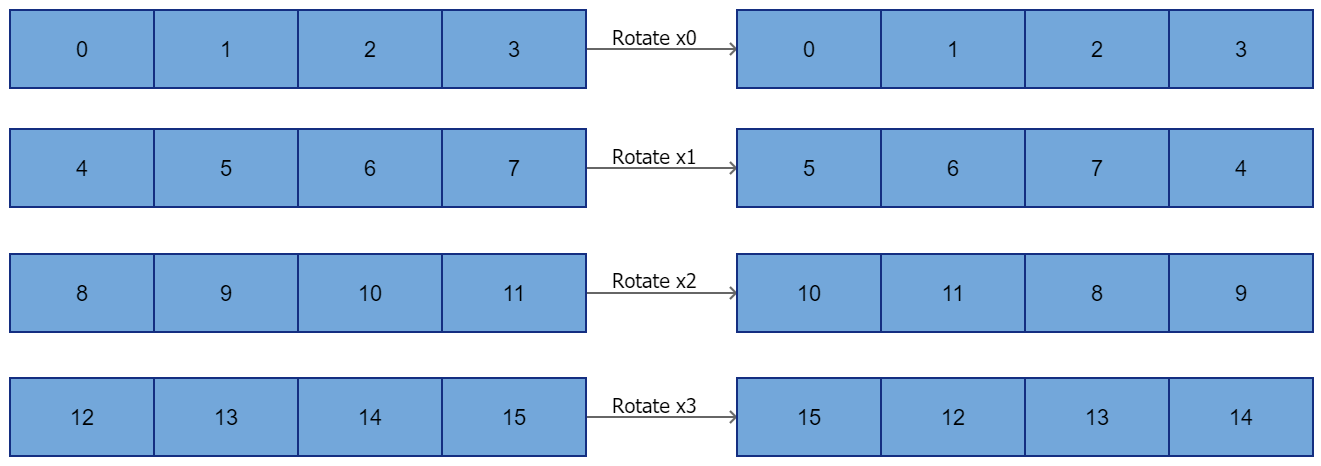
\includegraphics[width=\textwidth]{images/shiftrow.png}
    \caption{Rotationsmuster der \texttt{ShiftRow}-PROC}
    \label{fig:shiftrow}
\end{figure}

Wie zu erkennen, wird die erste Zeile des Datensatzes nicht verändert. Der Block aus 16 Einheiten wird in vier gedachte Zeilen zerlegt. Die zweite Zeile dagegen bekommt eine Rotation einmal nach Links. Somit steht die Stelle 7 nun an der ehemaligen Stelle 4. Dadurch rückt diese (4) an die Stelle 5 und so weiter.

Zeile 3 wird um 2 Stellen und die 4. Zeile um 3 Stellen rotiert. Dieses Muster wird 4x durchlaufen, da unser 64 Zeichen langer Text aus dem \asm{TastaturBuffer} in 4 Blöcke à 16 Einträge perfekt geteilt werden kann.
% TODO v2.0.0: Der ShiftRow-Fix (CMP CX, 5) sorgt dafuer, dass tatsaechlich alle
% vier Bloecke bearbeitet werden (vorher nur drei).

\subsubsection{ShiftColumn (PROC)}
Diese \asm{PROC} setzt das Spaltenrechnen von AES um. Dabei wird mithilfe der C-Matrix eine Verrechnung der einzelnen Spalten vorgenommen, da man sich hier wieder die Blöcke aus 16 Einträgen vorstellen muss. Nachfolgende Grafik soll dies zeigen:

\begin{figure}[!htbp]
    \centering
    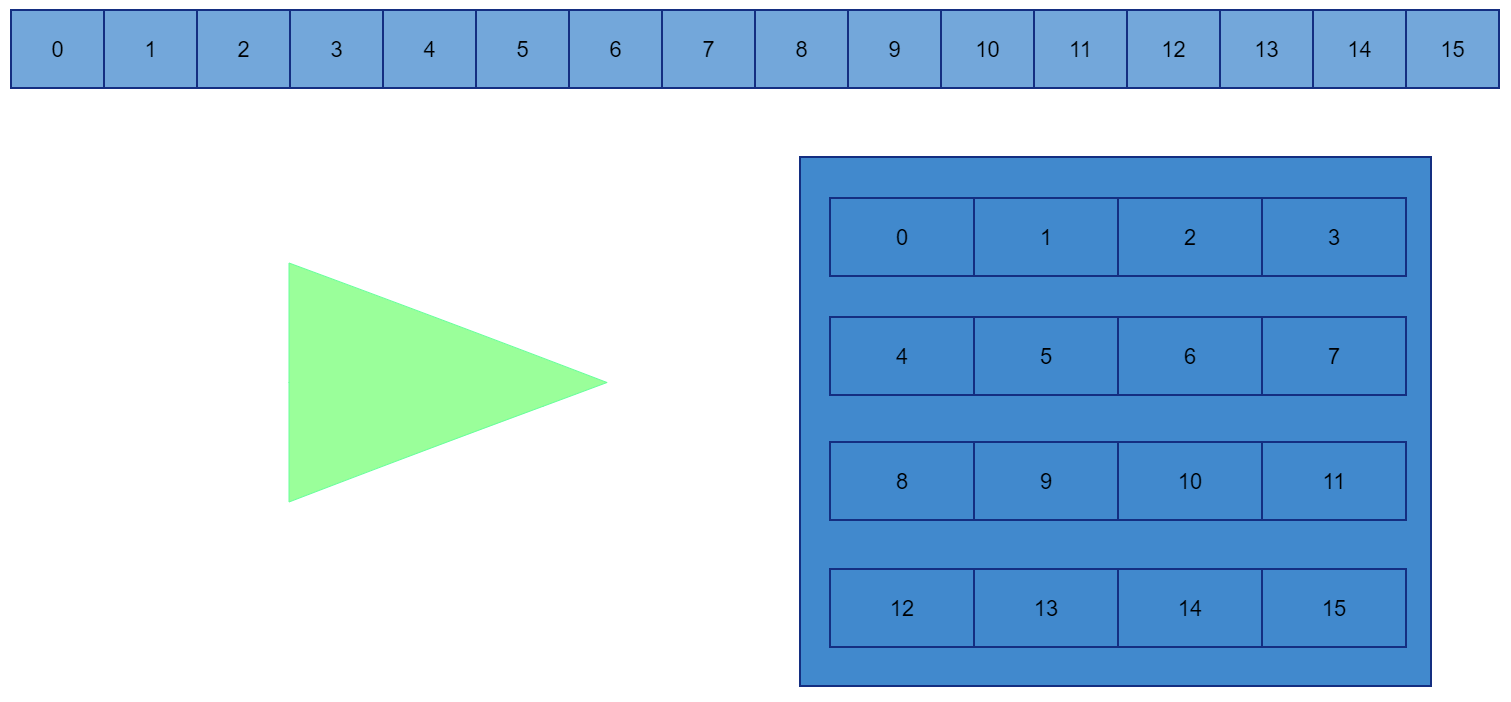
\includegraphics[width=\textwidth]{images/shiftcolumn_1.png}
    \caption{ShiftColumn: Die Blöcke aus 16 Einträgen werden spaltenweise verrechnet}
    \label{fig:shiftcolumn-1}
\end{figure}

Bei einem Durchlauf einer Spalte werden nun die Werte \glqq 0\grqq, \glqq 4\grqq, \glqq 8\grqq, \glqq 12\grqq{} mit der C-Matrix nach den mathematischen Gesetzen verrechnet.

\begin{figure}[!htbp]
    \centering
    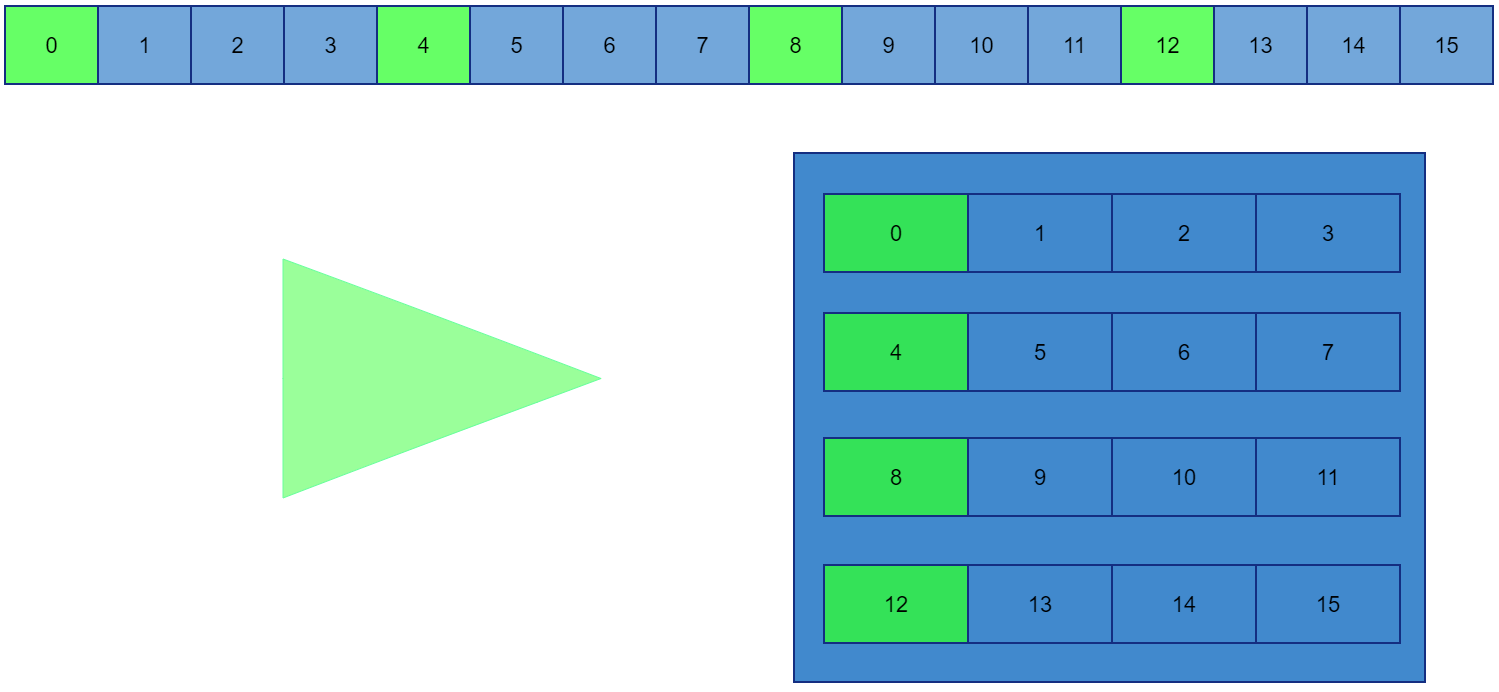
\includegraphics[width=\textwidth]{images/shiftcolumn_2.png}
    \caption{ShiftColumn: Verrechnung einer Spalte (Einträge 0, 4, 8 und 12)}
    \label{fig:shiftcolumn-2}
\end{figure}

Somit werden mit einer Rechnung pro C-Matrix 4 Einträge manipuliert. Für den gesamten \asm{TastaturBuffer} muss also die Multiplikation mit der C-Matrix insgesamt 16x angewendet werden.

\subsubsection{MalZweiProc (PROC)}
Hier findet eine Fallunterscheidung statt, welche den Wert als größer 127 oder kleiner gleich 127 erkennt. Sollte er kleiner sein, so wird er durch ein \asm{SHL} (shift left = schiebe nach links) mit 2 multipliziert. Andernfalls wird eine XOR-Operation mit $283_{\text{dez}}$ durchgeführt und anschließend mal 2 gerechnet. Ein Aufruf dieser \asm{PROC} erfolgt über die \asm{ShiftColumn} an mehreren Stellen.
% TODO v2.0.0: MalZweiPROC wurde korrigiert (SHL AL,1; bei Ueberlauf XOR 1Bh) und
% um GFMulPROC (allgemeine GF(2^8)-Multiplikation) ergaenzt.

%------------------------------------------------------------------------------
\subsection{ENTS.asm}
\subsubsection{SBOXSubstitution\_1 (PROC)}
In dieser \asm{PROC} wird der gesamte \asm{TastaturBuffer} mithilfe der invertierten \asm{SBOX} substituiert. Wie die Substitution an sich abläuft, ist im Abschnitt~\ref{sec:sbox} \nameref{sec:sbox} beschrieben.

\subsubsection{ShiftRow\_1 (PROC)}
Beim Aufruf dieser \asm{PROC} wird mit dem zeilenweisen Rotieren der Inhalte begonnen. Dieses Rotieren findet nach folgendem Muster statt:

\begin{figure}[!htbp]
    \centering
    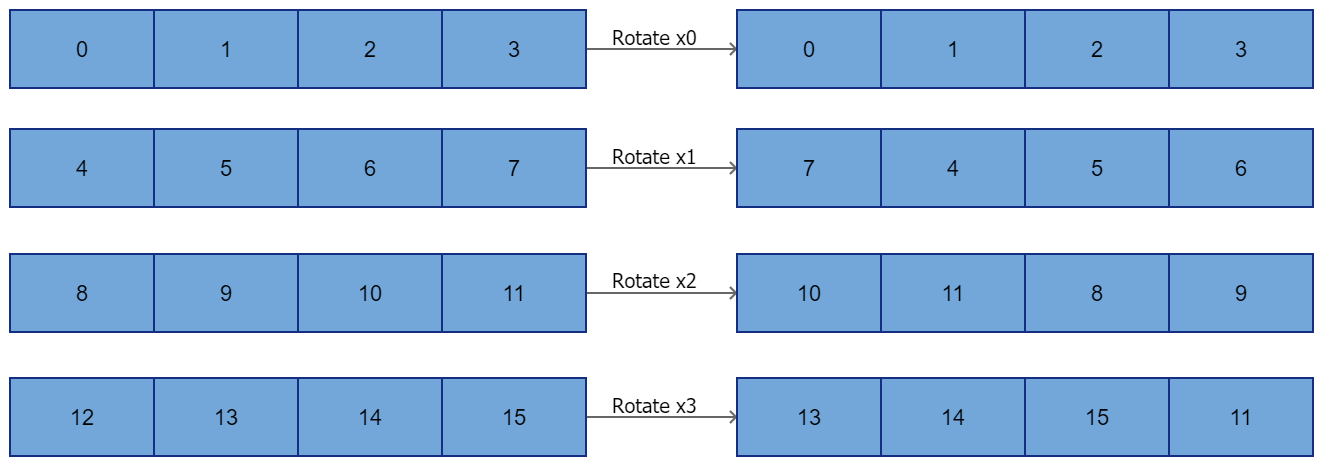
\includegraphics[width=\textwidth]{images/shiftrow_invers.png}
    \caption{Rotationsmuster der \texttt{ShiftRow\_1}-PROC (inverse Variante)}
    \label{fig:shiftrow-invers}
\end{figure}

Aus der Grafik ist erkennbar, dass die erste Zeile keine Rotation zu verzeichnen hat. Die Zweite dagegen hat einen \asm{ShiftRight} (schiebe nach rechts) mit Sicherung des Inhaltes 7 und Einschub von links an die Stelle 4.

Bei Zeile 3 wird eine 2fache Rotation durchgeführt. Somit stehen alle Einträge zwei Plätze weiter rechts. Auch hier werden die raus fallenden Inhalte von links wieder eingefügt, wie es bei einer Rotation definiert ist.

Bei der letzten Zeile findet eine Verschiebung um 3 statt, damit jedes Verschiebemuster in den 4 Zeilen einmal stattgefunden hat.

\subsubsection{ShiftColumn\_1 (PROC)}
% TODO v2.0.0: ShiftColumn_1 wurde in Version 2.0.0 neu geschrieben (inverse
% MixColumns mit InvMixMatrix). Der folgende Absatz beschreibt den Stand 1.x.
Leider nicht funktionsfähig\ldots{}

Hier soll die Verrechnung mit der inversen C-Matrix stattfinden:
\[
    \begin{pmatrix}
        \mathrm{E} & \mathrm{B} & \mathrm{D} & 9 \\
        9 & \mathrm{E} & \mathrm{B} & \mathrm{D} \\
        \mathrm{D} & 9 & \mathrm{E} & \mathrm{B} \\
        \mathrm{B} & \mathrm{D} & 9 & \mathrm{E}
    \end{pmatrix}
\]

Wie schon bei der nicht inversen Variante wird eine einzelne (gedachte) Spalte mit einer Zeile der Matrix verrechnet. Die einzelnen Einträge werden multipliziert und diese dann zum Schluss durch ein \asm{XOR} logisch verknüpft.

%------------------------------------------------------------------------------
\subsection{SBOX.asm}\label{sec:sbox}
In dieser asm-Datei werden zwei elementare Arrays angelegt. Das Erste beinhaltet die \asm{SBOX}, welche zum Verschlüsseln benötigt wird, während das Zweite schlicht die inverse \asm{SBOX} enthält (zum Entschlüsseln).

Das Grundprinzip in der Anwendung einer \asm{SBOX} besteht daraus, dass mithilfe des zu wechselnden Wertes die Stelle im Array ermittelt wird, wo der neue (substituierte) Wert dann herausgenommen wird.

Als Beispiel wäre die Eingabe $36_{\text{hex}}$ gegeben. Dies entspricht dem dezimal Wert $54_{\text{dez}}$ und verweist somit auf die 54.\ Stelle im Array, also dem Index $53_{\text{dez}}$ des Arrays. An dieser Stelle befindet sich der vordefinierte Wert $102_{\text{dez}}$ -- was $66_{\text{hex}}$ entspricht. Bei der Substitution wird nun dieser Wert ($66_{\text{hex}}$) mit dem vorherigen Wert ($36_{\text{hex}}$) ersetzt.

Bei der inversen \asm{SBOX} erfolgt dieses Ersetzen der Werte genau nach dem selben Schema.

%------------------------------------------------------------------------------
\subsection{config.asm}
In dieser Datei finden sich alle Variablen. Aufgelistet wären das:

% Hinweis: Im PDF waren die Beschreibungen von Hauptbildschirm4_Ergebnis und
% Hauptbildschirm5_Ergebnis vertauscht. Laut Quelltext (Ver_Code.asm setzt
% BildschirmVar auf 4, Ent_Code.asm auf 5) gehoert 4 zur Verschluesselung.
\begin{longtable}{@{}p{3.8cm}p{1.8cm}p{8.2cm}@{}}
    \caption{Variablen der \texttt{config.asm}}\label{tab:config}\\
    \toprule
    \textbf{Name} & \textbf{Datentyp} & \textbf{Beschreibung} \\
    \midrule
    \endfirsthead
    \toprule
    \textbf{Name} & \textbf{Datentyp} & \textbf{Beschreibung} \\
    \midrule
    \endhead
    \midrule
    \multicolumn{3}{r}{\small\emph{weiter auf der nächsten Seite}} \\
    \endfoot
    \bottomrule
    \endlastfoot
    \asm{Rundenanzahl} & DB & Beinhaltet die Anzahl der Runden. Damit kann man leichter dann aus z.\,B.\ 10 Runden 5 machen. \\
    \asm{bool_Ent_Ver} & DB & Beinhaltet die Variable, die genutzt wird, um festzuhalten, ob Entschluesseln, Verschluesseln oder keine der Schaltflächen gedrückt wurde. \\
    \asm{ESC_Code} & DB & \asm{1Bh} => Tastaturcode von der ESC-Taste. Für bessere Lesbarkeit im Code. \\
    \asm{Entertaste_Code} & DB & \asm{0Dh} => Tastaturcode von der Enter-Taste. Für bessere Lesbarkeit im Code. \\
    \asm{Video_Seg} & DW & Adresse vom Videosegment. Damit der Videomodus 3 auch alles korrekt printed. \\
    \asm{oldIOFF} & DW & Offset der ehemaligen Interrupt-Service-Routine. \\
    \asm{oldISeg} & DW & Segmentadresse der ehemaligen Interrupt-Service-Routine. \\
    \asm{Hauptbildschirm} & DB & Beinhaltet den String, der das Hauptmenü beinhaltet. (siehe \asm{config.asm}) \\
    \asm{Hauptbildschirm2} & DB & Beinhaltet den String, der den Bildschirm für die Eingabe zum Entschlüsseln beinhaltet (siehe \asm{config.asm}) \\
    \asm{Hauptbildschirm3} & DB & Beinhaltet den String, der den Bildschirm für die Eingabe zum Verschlüsseln beinhaltet. (siehe \asm{config.asm}) \\
    \asm{Hauptbildschirm4_Ergebnis} & DB & Beinhaltet den String, der den Bildschirm für die Ausgabe des Verschlüsseln-Ergebnisses beinhaltet. (siehe \asm{config.asm}) \\
    \asm{Hauptbildschirm5_Ergebnis} & DB & Beinhaltet den String, der den Bildschirm für die Ausgabe des Entschlüsseln-Ergebnisses beinhaltet. (siehe \asm{config.asm}) \\
    \asm{BildschirmVar} & DB & Hier wird eingetragen, welcher der 4 (nicht Haupt-)Bildschirme zu zeichnen sind. Diese Variable wird von der \asm{BildschirmProcX} verwendet. \\
    \asm{EntR1_L} & DW & =499 Beinhaltet die Blocknummer (*2) der oberen Zeile vom ENTSCHLUESSELN (Links) \\
    \asm{EntR1_R} & DW & =535 Beinhaltet die Blocknummer (*2) der oberen Zeile vom ENTSCHLUESSELN (Rechts) \\
    \asm{EntR2_L} & DW & =659 Beinhaltet die Blocknummer (*2) der mittleren Zeile vom ENTSCHLUESSELN (Links) \\
    \asm{EntR2_R} & DW & =695 Beinhaltet die Blocknummer (*2) der mittleren Zeile vom ENTSCHLUESSELN (Rechts) \\
    \asm{EntR3_L} & DW & =819 Beinhaltet die Blocknummer (*2) der unteren Zeile vom ENTSCHLUESSELN (Links) \\
    \asm{EntR3_R} & DW & =855 Beinhaltet die Blocknummer (*2) der unteren Zeile vom ENTSCHLUESSELN (Rechts) \\
    \asm{VerR1_L} & DW & =581 Beinhaltet die Blocknummer (*2) der oberen Zeile vom VERSCHLUESSELN (Links) \\
    \asm{VerR1_R} & DW & =617 Beinhaltet die Blocknummer (*2) der oberen Zeile vom VERSCHLUESSELN (Rechts) \\
    \asm{VerR2_L} & DW & =741 Beinhaltet die Blocknummer (*2) der mittleren Zeile vom VERSCHLUESSELN (Links) \\
    \asm{VerR2_R} & DW & =777 Beinhaltet die Blocknummer (*2) der mittleren Zeile vom VERSCHLUESSELN (Rechts) \\
    \asm{VerR3_L} & DW & =901 Beinhaltet die Blocknummer (*2) der unteren Zeile vom VERSCHLUESSELN (Links) \\
    \asm{VerR3_R} & DW & =937 Beinhaltet die Blocknummer (*2) der unteren Zeile vom VERSCHLUESSELN (Rechts) \\
    \asm{TastaturBuffer} & DB & Hier werden die Hex-Werte der Zeichen gespeichert, welche per Tastatureingabe erkannt wurden. \\
    \asm{TastaturBufferOrg} & DB & Dient als Sicherung der Eingabe, um die Ausgabe des Originaltextes zu gewährleisten. \\
    \asm{Konstante} & DB & $=5F_{\text{hex}}$ \textbar{} Ist die vordefinierte Initialkonstante. \\
    \asm{Rundenkonstante} & DB & Ermittelte sich aus der durch \asm{ROL} veränderten vorherigen Rundenkonstante. \\
    % TODO v2.0.0: Rundenschluessel_0 -> Der Hinweis "nicht ueberschreibbar" gilt weiterhin
    % fuer den Standardschluessel; die Eingabe schreibt nur in Rundenschluessel_Expand.
    \asm{Rundenschluessel_0} & DB & Ist der fest implementierte Standardschlüssel, welcher während der Laufzeit auch nicht überschrieben werden kann. \\
    \asm{Rundenschluessel_Expand} & DB & Hier wird der \asm{Rundenschluessel_0} reinkopiert. Bei einer Benutzereingabe eines eigenen Schlüssels, werden nur hier die entsprechenden Einträge verändert. Ebenfalls die erweiterten Schlüssel (siehe \asm{Schluesselexpansion}) werden hier abgelegt. \\
    \asm{ShiftZwSpeicher} & DB & Wird benötigt für die Arbeit der \asm{ShiftRow} und seinem Pendant \asm{ShiftRow_1}. \\
    \asm{ShiftBXZwSpeicher} & DW & Da ein Index-Register nicht mit einem Halb-Register (H oder L) verglichen werden kann, wird das \asm{BX}-Register hier genutzt, was durch den internen Ablauf jedoch an einigen Stellen zwischengespeichert werden muss. \\
    \asm{ShiftColumnZW} & DW & Sichert die Zwischenergebnisse aus der \asm{ShiftColumn} \& \asm{ShiftColumn_1}. \\
    \asm{ShiftColumnZW2} & DW & Sichert die Zwischenergebnisse aus der \asm{ShiftColumn} für die Spaltenrechnung, sonst gäbe es Rechenfehler da Werte überschrieben werden. \\
\end{longtable}

Die in der \asm{config.asm} abgelegten Bildschirme (Hauptbildschirm 2 bis 5) sehen im Programm wie folgt aus:

\begin{figure}[!htbp]
    \centering
    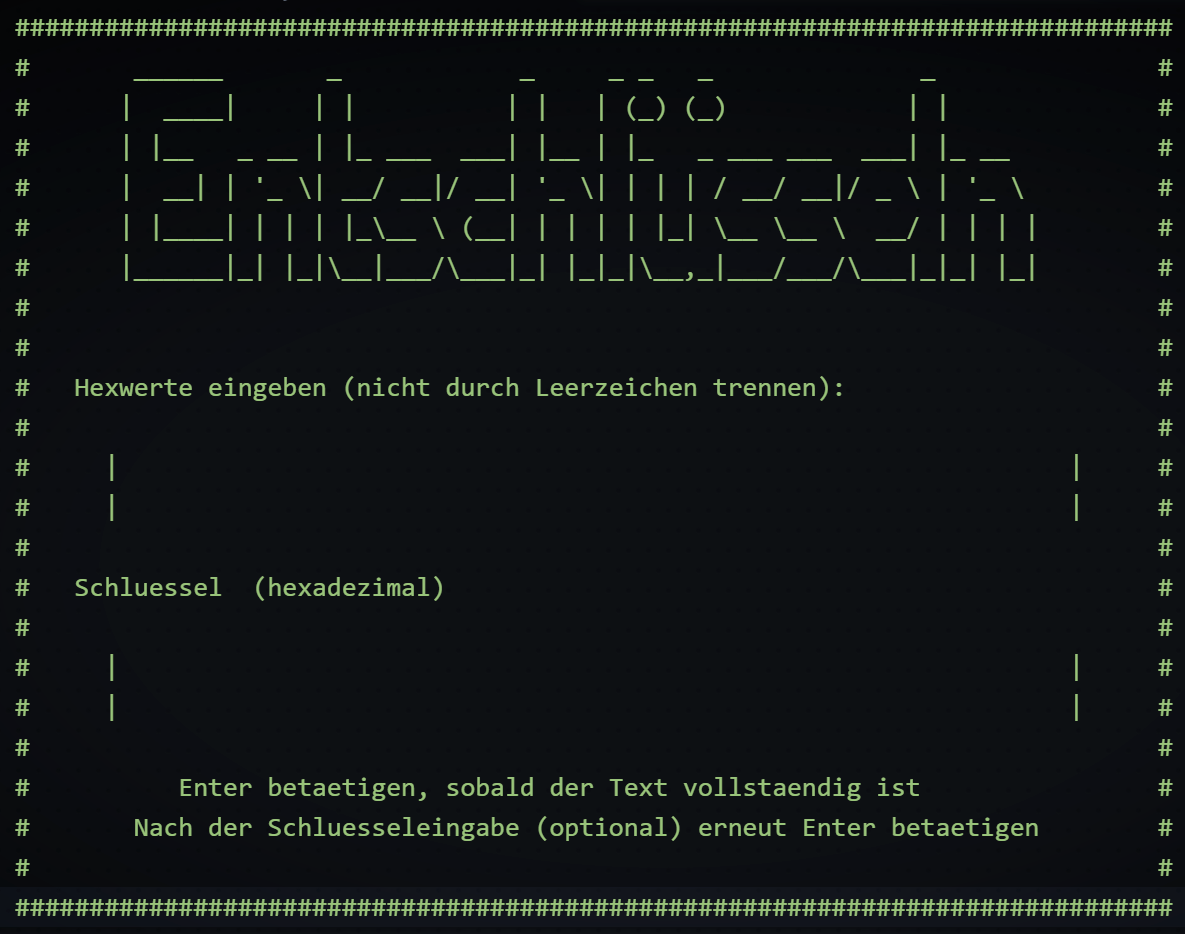
\includegraphics[width=0.7\textwidth]{images/bildschirm_ent_eingabe.png}
    \caption{\texttt{Hauptbildschirm2}: Eingabe zum Entschlüsseln}
    \label{fig:bs2}
\end{figure}

\begin{figure}[!htbp]
    \centering
    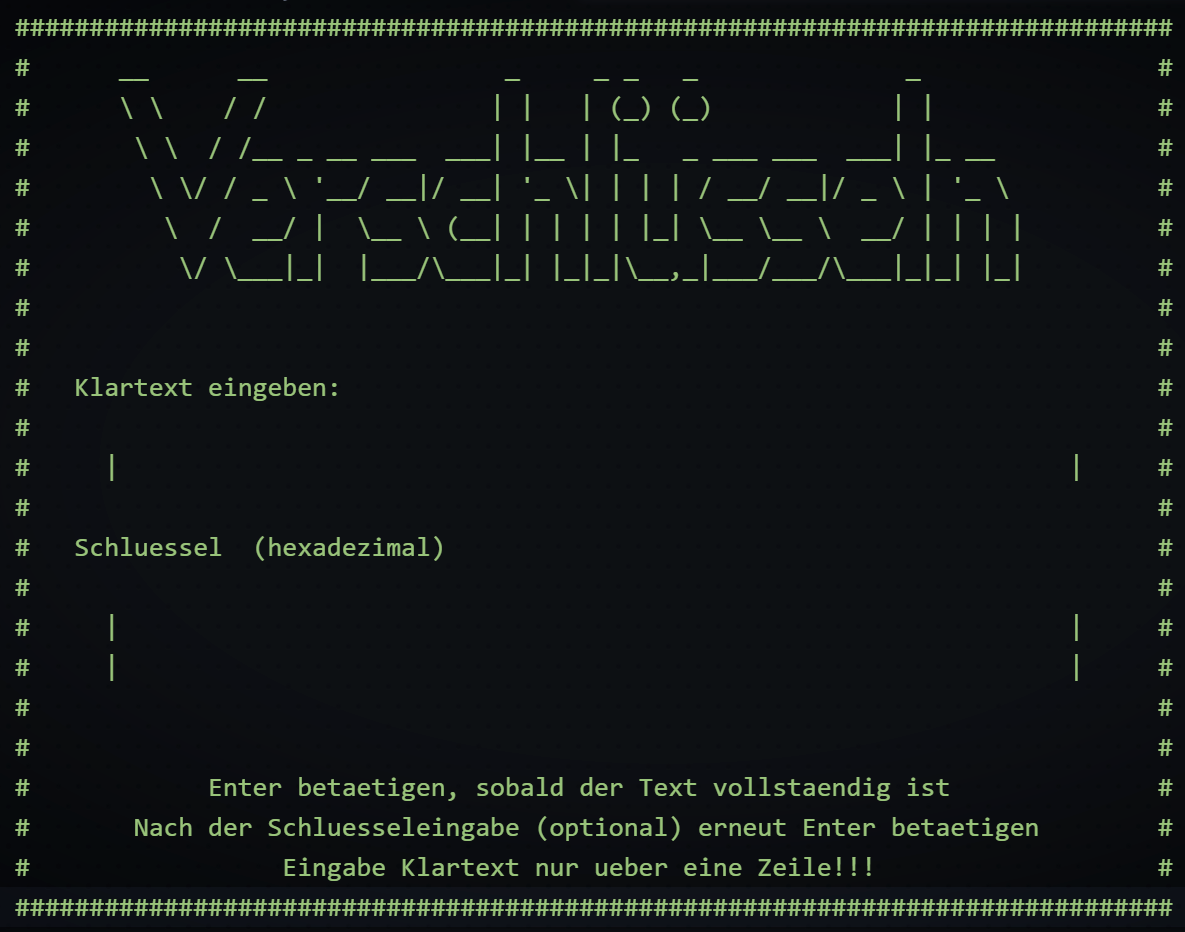
\includegraphics[width=0.7\textwidth]{images/bildschirm_ver_eingabe.png}
    \caption{\texttt{Hauptbildschirm3}: Eingabe zum Verschlüsseln}
    \label{fig:bs3}
\end{figure}

\begin{figure}[!htbp]
    \centering
    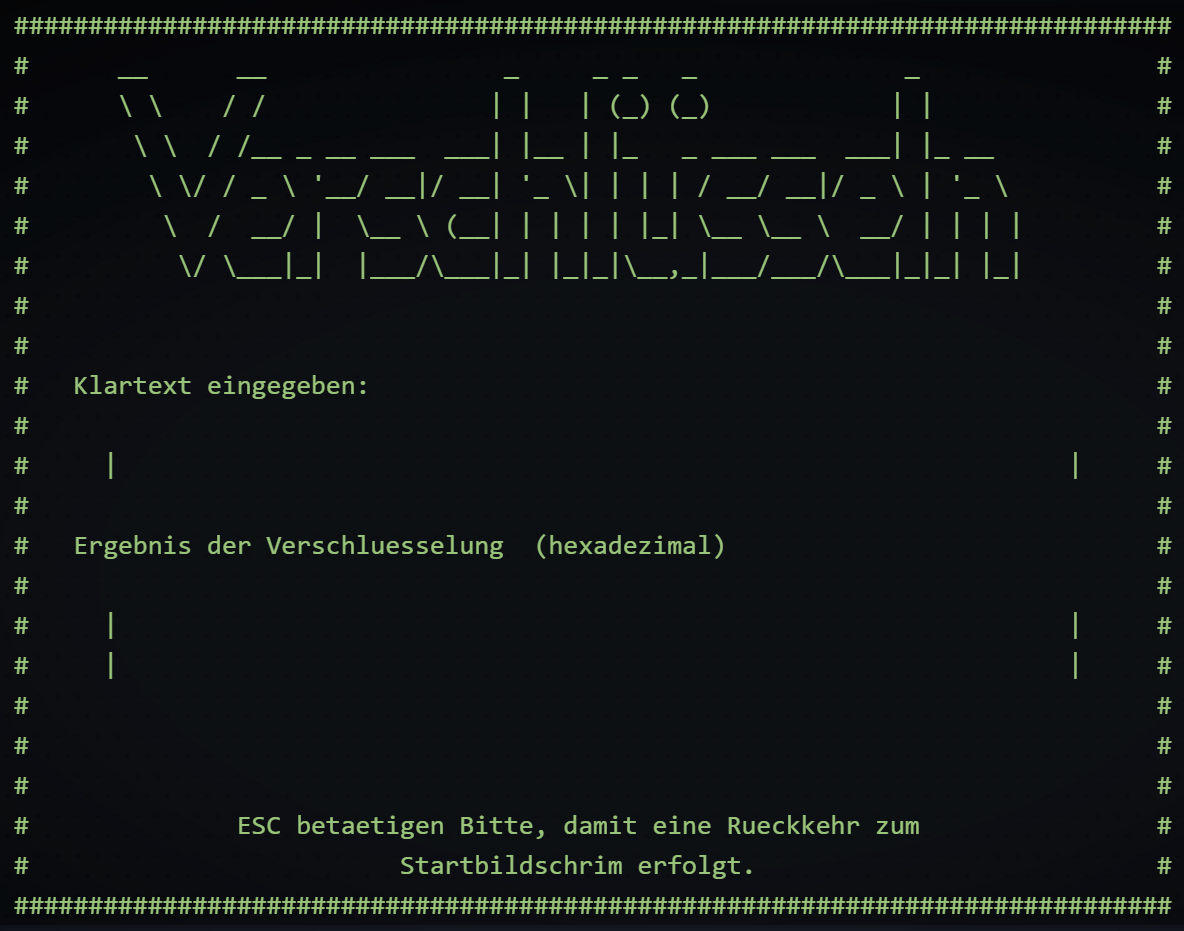
\includegraphics[width=0.7\textwidth]{images/bildschirm_ver_ergebnis.png}
    \caption{\texttt{Hauptbildschirm4\_Ergebnis}: Ausgabe der Verschlüsselung}
    \label{fig:bs4}
\end{figure}

\begin{figure}[!htbp]
    \centering
    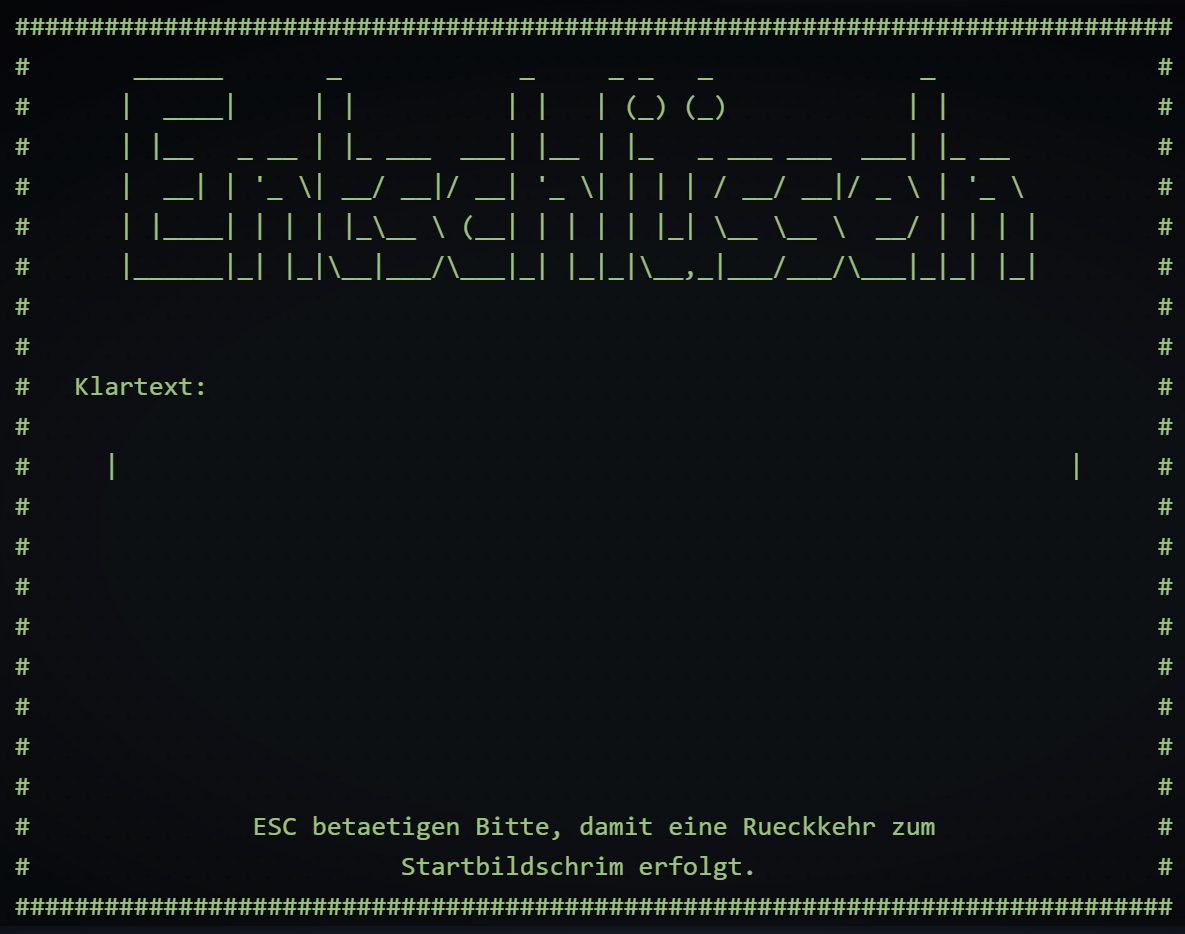
\includegraphics[width=0.7\textwidth]{images/bildschirm_ent_ergebnis.png}
    \caption{\texttt{Hauptbildschirm5\_Ergebnis}: Ausgabe der Entschlüsselung}
    \label{fig:bs5}
\end{figure}

%------------------------------------------------------------------------------
\subsection{ISR.asm}
Diese gesamte Datei beinhaltet einen rein zur Demonstration erstellten Codesatz, um zu beweisen, dass uns bekannt ist, wie die Erstellung und Einschreibung einer eigenen Interrupt-Service-Routine (kurz: ISR) ablaufen muss.

\subsubsection{ISR1Ch (Label)}
Hier wird beschrieben, was in der eigens erstellten ISR ablaufen soll. Unspektakulärerweise ist dies bei diesem Programm ein \asm{NOP}-Befehl.

\subsubsection{EigeneISR (PROC)}
Mit dieser \asm{PROC} wird das Eintragen der selbst erstellten ISR durchgeführt. Näheres dazu ist im Quelltext-Kommentar zu lesen.

\subsubsection{ISR\_Zuruecksetzten (PROC)}
Beim Aufruf dieser \asm{PROC} erfolgt das Zurücksetzen der \asm{ISR-1Ch}, damit das Programm beendet werden kann.

%------------------------------------------------------------------------------
\subsection{BildPROC.asm}
Diese zwei \asm{PROC}s haben die Funktionalität, das Zeichnen der Bildschirme, welche in der \asm{config.asm} definiert sind, auszuführen.

\subsubsection{HauptbildschirmProc (PROC)}
Sobald der \asm{CALL} dieser \asm{PROC} erfolgt, wird das Videosegment in \asm{ES} geladen, damit für den Videomodus 3 festgelegt wird, wo er zu zeichnen hat. Somit wird der Hauptbildschirm dargestellt (Näheres in den Kommentaren der Befehlszeilen). Abschließend wird die, für die interne Verarbeitung benötigte, Variable \asm{bool_Ent_Ver} auf 3 gesetzt (also nichts tun). Daraufhin geschieht der Rücksprung zum Programm über ein \asm{RET}.

\begin{figure}[!htbp]
    \centering
    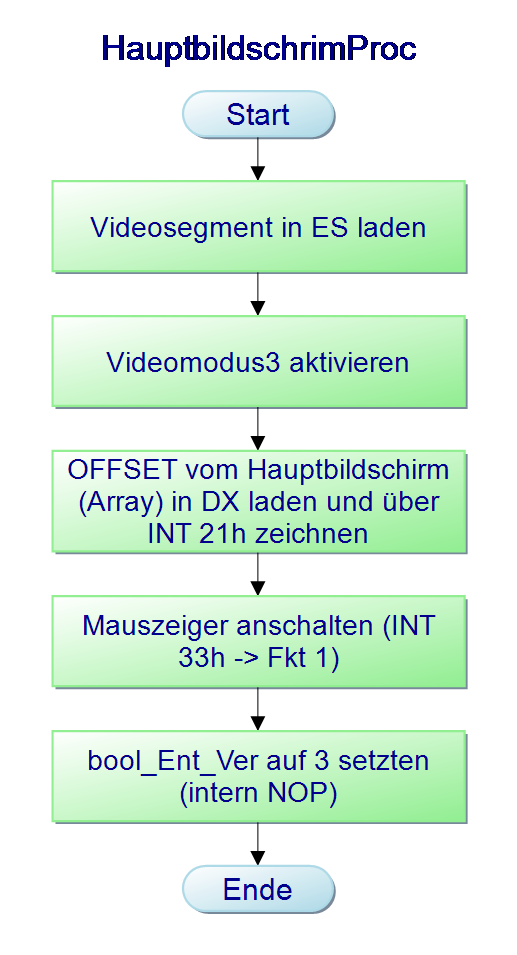
\includegraphics[height=0.5\textheight,keepaspectratio]{images/pap_hauptbildschirmproc.png}
    \caption{Programmablaufplan der \texttt{HauptbildschirmProc}}
    \label{fig:pap-hauptbildschirmproc}
\end{figure}

\subsubsection{BildschirmProcX (PROC)}\label{sec:bildschirmprocx}
Nach dem Aufruf dieser \asm{PROC}, wird zunächst das Videosegment in \asm{ES} geladen. Anschließend wird der Bildschirm, durch die erneute Einstellung des Videomodus 3 geleert und zum abermaligen Zeichnen von Inhalten vorbereitet. Näheres dazu in den Kommentaren bei den Befehlszeilen.

Als erstes erfolgt ein Vergleich der Variable \asm{BildschirmVar} auf den Wert 2. Sollte dieser erfolgreich sein, so wird der \asm{Hauptbildschirm2} gezeichnet (Entschlüsseln-Eingabe). Nach der Ausführung (graphische Darstellung des Bildschirms) springt das Programm zum Ende der \asm{PROC} und kehrt zum vorherigen Programmabschnitt über ein \asm{RET} zurück. Sollte der Vergleich der \asm{BildschirmVar} mit 2 negativ ausgefallen sein, so erfolgt nun ein \asm{CMP} auf den Inhalt mit 3. Hier wird nach dem selben Muster der Aufruf des \asm{Hauptbildschirm3} (Verschlüsseln-Eingabe) erfolgen, mit anschließendem Sprung zum \asm{BildschirmEnde} (Label).

Bei erneut fehlgeschlagenem Test, erfolgt ein Vergleich auf den Wert 4. Dieser codiert den \asm{Hauptbildschirm4_Ergebnis} (Verschlüsseln-Ausgabe). Als letzter Vergleich wird die Variable \asm{BildschirmVar} mit dem Wert 5 abgeglichen. Dieser bringt den \asm{Hauptbildschirm5_Ergebnis} (Entschlüsseln-Ausgabe) zum Zeichnen.

Sollten durch einen Fehler im Programm oder durch externe Einflüsse die \asm{BildschirmVar} keinen der hier 4 codierten Zustände haben, so wird in der \asm{PROC} das Zeichnen an sich vernachlässigt. Stattdessen findet ein \asm{JMP} zum \asm{BildschirmEnde} (Label) statt. Das Unterprogramm \asm{BildschirmProcX} führt ein \asm{RET} durch und wird beendet.

\begin{figure}[!htbp]
    \centering
    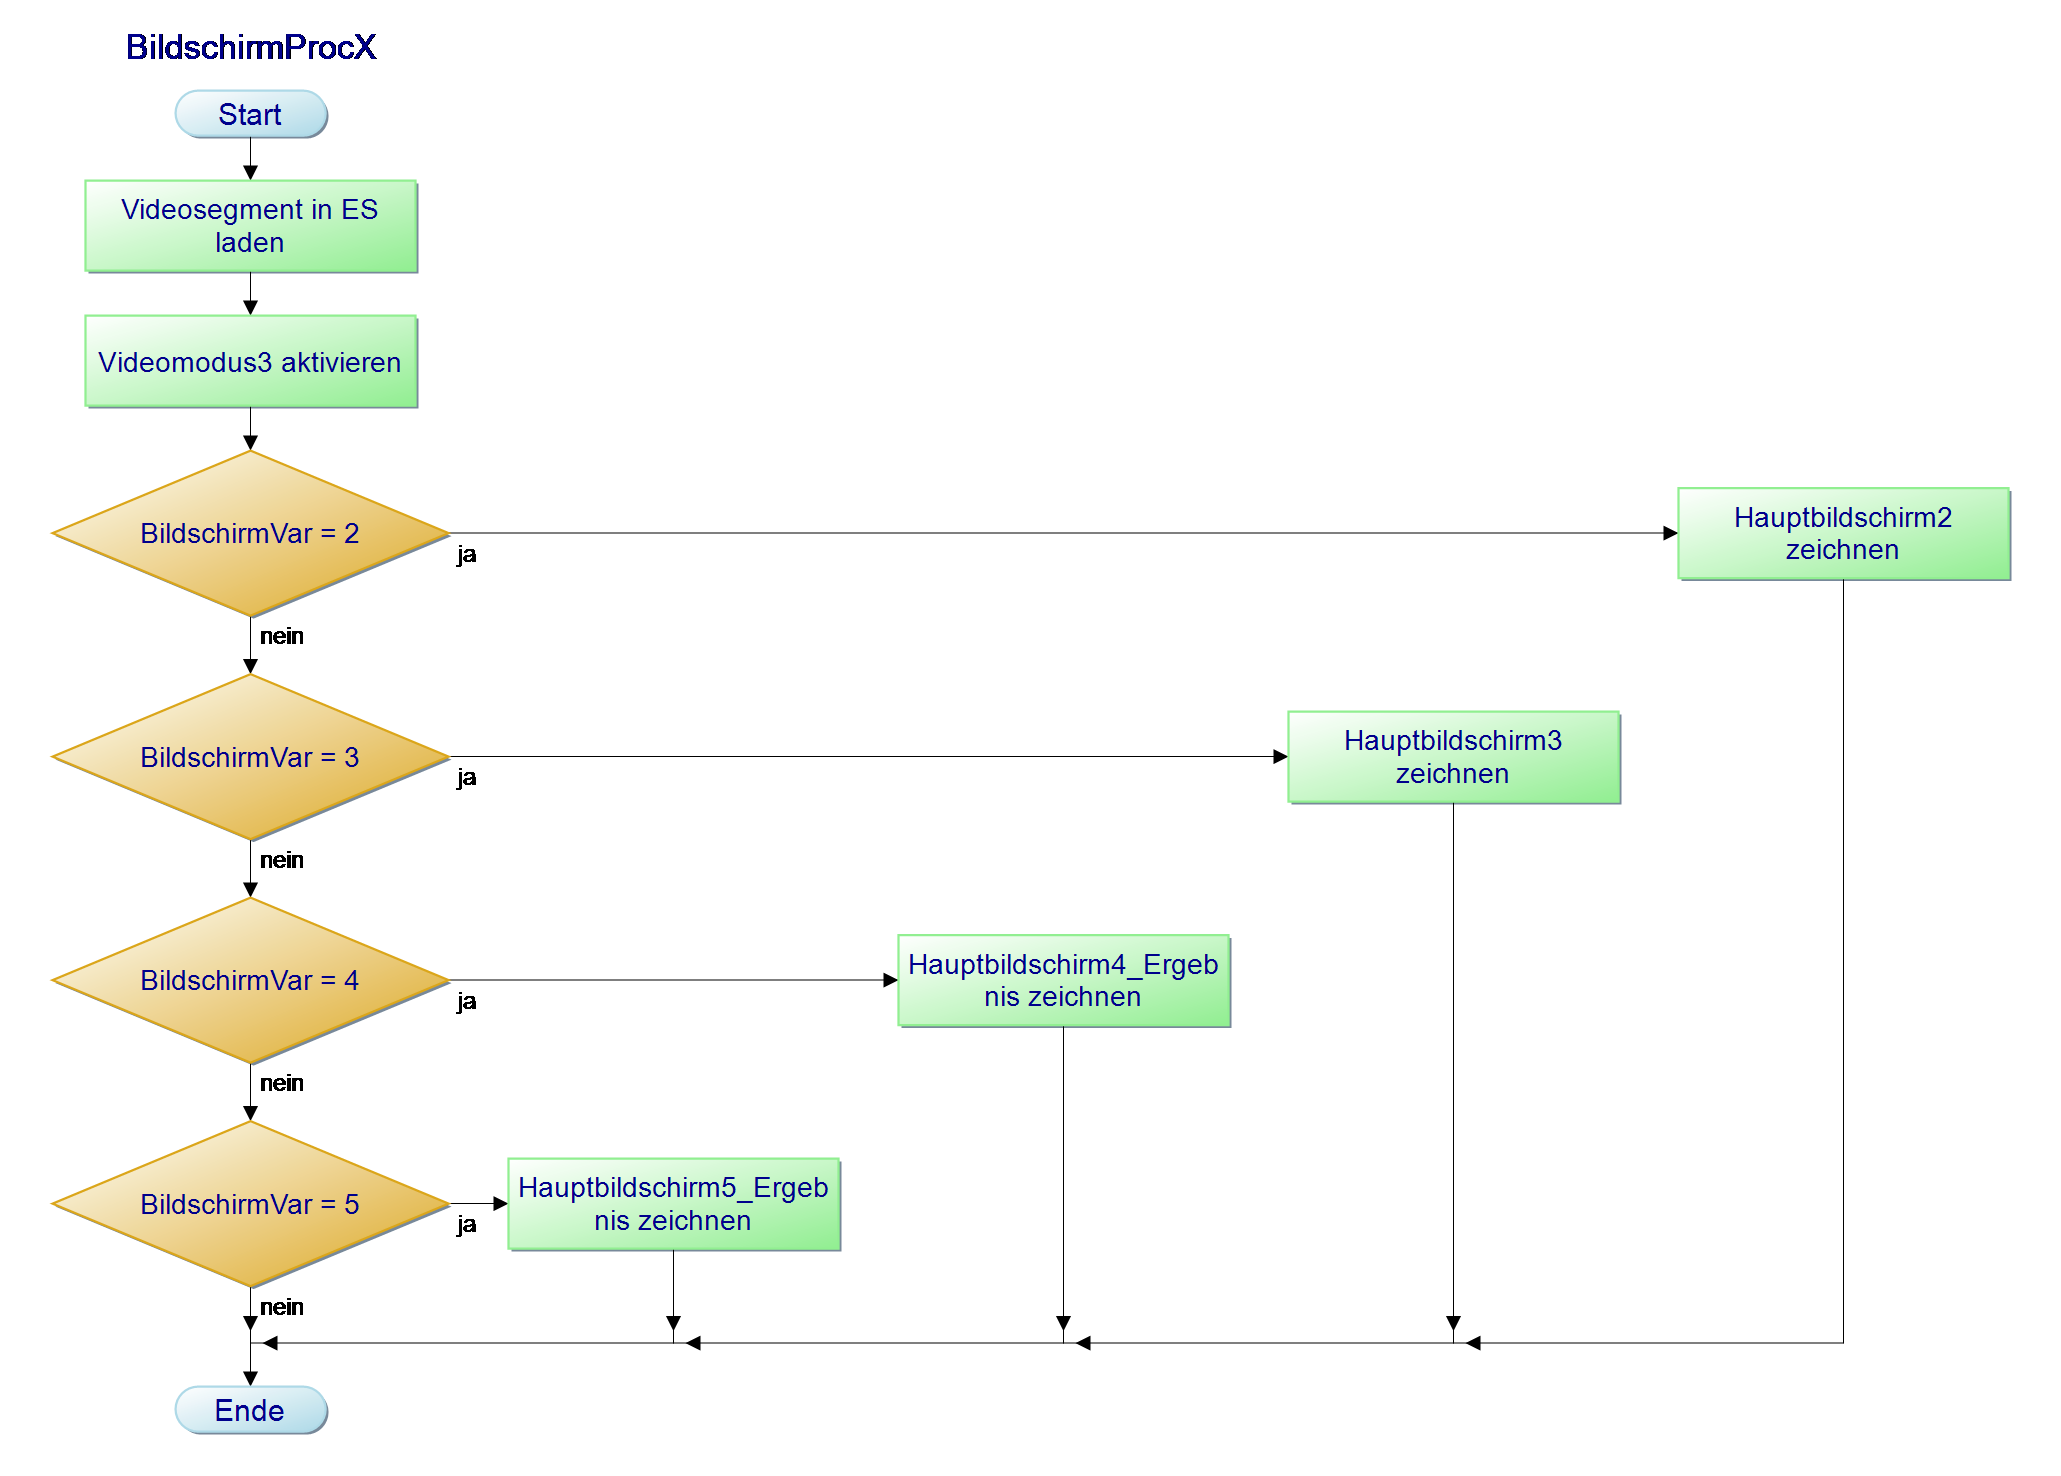
\includegraphics[width=\textwidth]{images/pap_bildschirmprocx.png}
    \caption{Programmablaufplan der \texttt{BildschirmProcX}}
    \label{fig:pap-bildschirmprocx}
\end{figure}

    \newpage
    % Ehemals AES.pdf, Kapitel 3
\section{Batch-Dateien}\label{sec:batch}

\subsection{asmaes.bat}
Diese ausführbare Datei beinhaltet folgenden Befehlssatz:

\begin{lstlisting}[language={},caption={\texttt{asmaes.bat}},label={lst:asmaes}]
cd ASM
tasm aes.asm
tlink aes.obj
cd ..
\end{lstlisting}

Damit wird für den ungeübten Benutzer, aber auch für den Experten in der DOS-Box, das Kompilieren der ASM-Dateien leichter. Mit dem ersten Befehl wird eine obj- und eine map-Datei erstellt dank des TASM-Compilers. Danach wird mit dem \asm{tlink}-Befehl eine exe aus der obj-Datei erzeugt, welche als ausführbare Datei in der DOS-Box dann gestartet werden kann. Der Name steht für \emph{assembliereaes}.

\subsection{tdaes.bat}
Diese ausführbare Datei beinhaltet folgenden Befehlssatz:

\begin{lstlisting}[language={},caption={\texttt{tdaes.bat}},label={lst:tdaes}]
cd ASM
tasm aes.asm
tlink aes.obj
td aes.asm
cd ..
\end{lstlisting}

Hier erfolgt nach dem Erstellen der exe-Datei noch der Aufruf des Turbodebuggers. Hiermit soll dem Benutzer der Aufruf des Debuggers nach Änderungen im Quellcode zum Testen vereinfacht werden. Der Name steht hier für \emph{starteturbodebuggervonaes}.

\subsection{start.bat}
Diese ausführbare Datei beinhaltet folgenden Befehlssatz:

\begin{lstlisting}[language={},caption={\texttt{start.bat}},label={lst:start}]
cd ASM
tasm aes.asm
tlink aes.obj
aes.exe
cd ..
\end{lstlisting}

Mit dieser Datei, die ebenfalls für einen Entwickler vorgesehen ist, wird nach dem Assemblieren der Start des richtigen Programms, nicht im Debugger wie in der \asm{tdaes.bat}, ausgeführt. Dies soll das Testen in der Oberfläche zeitlich effektiver gestalten, falls Änderungen oder Erweiterungen eingefügt \& getestet werden. Der Name steht hier für \emph{starteaes}.

\subsection{AES.bat}
Diese ausführbare Datei beinhaltet folgenden Befehlssatz:

\begin{lstlisting}[language={},caption={\texttt{AES.bat}},label={lst:aesbat}]
cd ASM
aes.exe
cd ..
\end{lstlisting}

Mit dieser ausführbaren Datei soll für den Endbenutzer der Start in der DOS-Box erleichtert werden. Da ein ungeübter Benutzer sich im gesamten Verzeichnis und den dazugehörigen Dateien möglicherweise nur schwer zurechtfindet, ist diese Datei mit dem simplen Befehl versehen, die assemblierte exe zu starten.


    % ---- Weitere Dokumente (ehemals eigene PDFs) ----
    \newpage
    % Ehemals Anleitung.pdf
\section{Kurze Anleitung}\label{sec:anleitung}
\textit{Abschlussprojekt Modul \glqq Assemblerprogrammierung\grqq{} von Konstantin Blechschmidt \& Tim M.\ Kretzschmar}

Nach dem Start des Programms mittels \asm{start.bat} oder \asm{aes.bat} kann per Mausklick auf die \glqq Entschluesselung\grqq{} oder \glqq Verschluesselung\grqq{} Bereiche das jeweilige gestartet werden. Dazu findet nun die Eingabe der jeweiligen Texte statt. Bei der Verschlüsselung natürlich der Klartext und bei der Entschlüsselung der Hexadezimalwert des Chiffretextes.

Nun muss einmal die Enter-Taste betätigt werden.

Anschließend kann ein Schlüssel eingegeben werden. Dies muss aber nicht geschehen, da ein vordefinierter Schlüssel im Programm existiert. Bei dem Wunsch, einen eigenen Schlüssel zu verwenden, ist dieser ebenfalls hexadezimal einzugeben.

Nun muss erneut die Enter-Taste betätigt werden, wodurch die Ver-/Entschlüsselung beginnt und anschließend auf dem neugezeichneten Bildschirm ausgegeben wird.

Sollte am Ende oder zwischendurch der Wunsch zur Rückkehr zum Hauptbildschirm eintreten, so ist dies mit der Betätigung der ESC-Taste jederzeit realisierbar.

\subsection*{Hinweise}
\begin{itemize}[noitemsep]
    \item Die hexadezimale Eingabe akzeptiert die Ziffern 0 bis 9 und groß A bis F.
    \item Der verschlüsselte Text erscheint hexadezimal, der entschlüsselte in ASCII-Zeichen.
\end{itemize}
% TODO v2.0.0: Eigene Schluessel werden seit 2.0.0 tatsaechlich verwendet
% (SchluesselInitialisieren wird nach der Eingabe aufgerufen).
              % Anleitung.pdf
    \newpage
    % Ehemals Deckblatt_und_Funktionalitaet.pdf
\section{Funktionalität und Erklärung}\label{sec:funktionalitaet}
\textit{Abschlussprojekt Modul \glqq Assemblerprogrammierung\grqq{} von Konstantin Blechschmidt \& Tim M.\ Kretzschmar}

\subsection*{Daten}
TASM; Prozessor .486; DOS-Box Version 0.74

\subsection*{Was geht}
% TODO v2.0.0: Seit 2.0.0 sind ShiftColumn invers (MixColumns-Inverse) implementiert,
% der S-Box-Tippfehler und ShiftRow fuer den 4. Block behoben (im Python-Modell
% verifiziert, TASM-Lauf steht noch aus).
\begin{itemize}[noitemsep]
    \item Grafik
    \item Mausklicken um Modi zu wechseln
    \item Eingabe/Ausgabe (Klartext (ASCII) und Hexadezimal)
    \item Beenden über \glqq ESC\grqq{} aus dem Hauptmenü heraus
    \item Schlüsselexpansion \& Schlüssel anwenden
    \item SBOX-Substitution \& inverse Version
    \item ShiftRow \& die inverse Version
    \item ShiftColumn
    \item Kompilieren, Debugger starten und einfaches Starten per Batch-Datei
\end{itemize}

\subsection*{Was geht nicht}
\begin{itemize}[noitemsep]
    \item Inverses ShiftColumn (haben wir leider nicht zum Laufen bekommen\ldots)\\
    mögl.\ Quelle: \cite{fips197}
\end{itemize}

\subsection*{Eidesstattliche Erklärung}
Hiermit bestätigen wir, Konstantin Blechschmidt \& Tim M.\ Kretzschmar, dass wir dieses Programm \glqq AES -- in TASM umgesetzt\grqq{} selbstständig und nur unter Angabe der genutzten Quellen erstellt und getestet haben.

\vspace{3mm}

\noindent
\begin{minipage}{\textwidth}
    \begin{minipage}[b]{0.52\textwidth}
        
\includegraphics[width=0.8\textwidth]{images/unterschrift_tim.png}
    \end{minipage}\hfill
    \begin{minipage}[b]{0.44\textwidth}
        Tim M.\ Kretzschmar\\(Wermsdorf, 03.08.2021)
    \end{minipage}

    \vspace{4mm}

    \begin{minipage}[b]{0.52\textwidth}
        
\includegraphics[width=0.7\textwidth]{images/unterschrift_konstantin.png}
    \end{minipage}\hfill
    \begin{minipage}[b]{0.44\textwidth}
        Konstantin Blechschmidt\\(Schkeuditz, 03.08.2021)
    \end{minipage}
\end{minipage}\par
        % Deckblatt_und_Funktionalitaet.pdf
    \newpage
    % Ehemals Entwurfsskizze.pdf
\section{Entwurfsskizze}\label{sec:entwurfsskizze}
\textit{Abschlussprojekt Modul \glqq Assemblerprogrammierung\grqq{} von Konstantin Blechschmidt \& Tim M.\ Kretzschmar}

% TODO v2.0.0: Teile dieses Entwurfs sind ueberholt (siehe Kommentare in
% funktionalitaet.tex).
Unser Programm kann in 2 Hauptbereiche mit je 2 Unterbereichen aufgeteilt werden.

\begin{description}[labelwidth=1cm,leftmargin=1.4cm,style=nextline]
    \item[I.\ Verschlüsselung]
        \begin{enumerate}[label=\alph*),noitemsep,topsep=0pt]
            \item graphische Ein-/Ausgabe Klartext und Ausgabe des Chiffretextes im Bildschirm + Schlüssel
            \item Abarbeitung der Verschlüsselung unter Zuhilfenahme der \asm{PROC}s aus der \asm{VERS.asm}
        \end{enumerate}
    \item[II.\ Entschlüsselung]
        \begin{enumerate}[label=\alph*),start=3,noitemsep,topsep=0pt]
            \item graphische Ein-/Ausgabe Chiffretext und Ausgabe des Klartextes im Bildschirm + Schlüssel
            \item Abarbeitung der Entschlüsselung unter Zuhilfenahme der \asm{PROC}s aus der \asm{ENTS.asm} und teilweise \asm{VERS.asm}
        \end{enumerate}
\end{description}

\begin{figure}[!htbp]
    \centering
    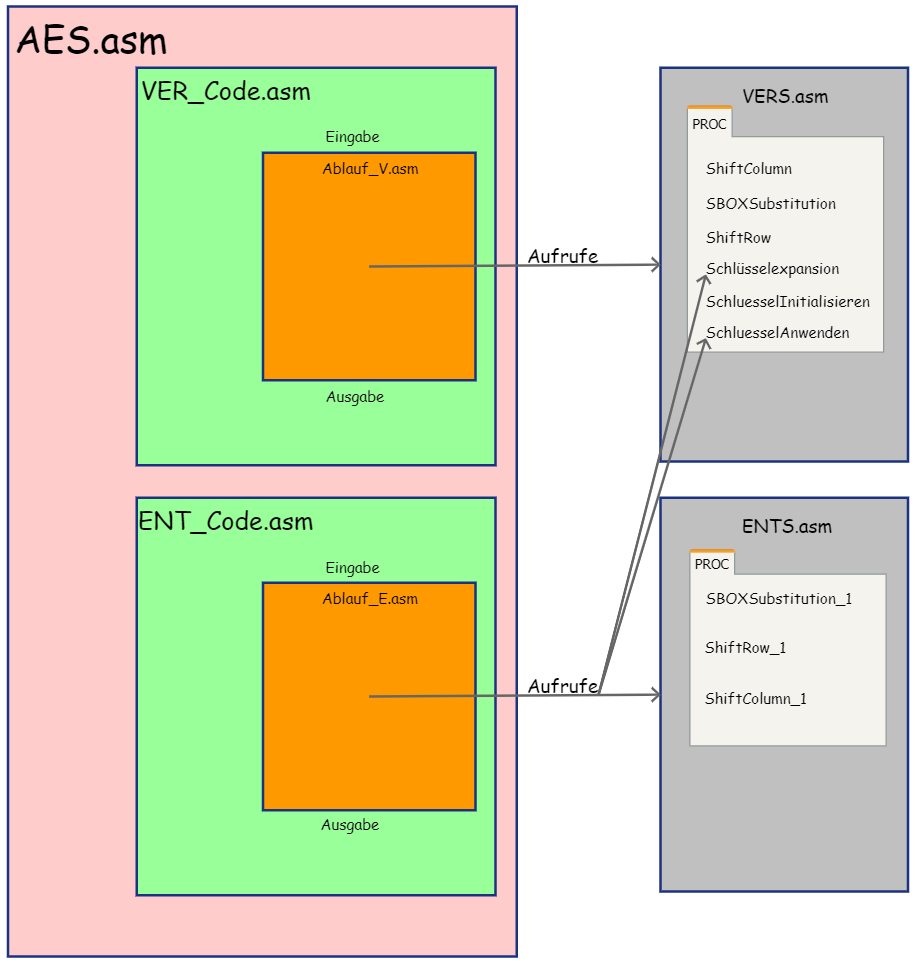
\includegraphics[height=0.5\textheight,keepaspectratio]{images/entw_zusammenspiel.png}
    \caption{Entwurf: Zusammenspiel der ASM-Dateien}
    \label{fig:entw-zusammenspiel}
\end{figure}

\begin{figure}[!htbp]
    \centering
    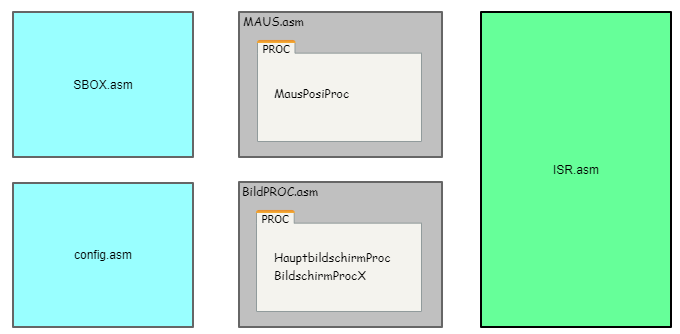
\includegraphics[width=0.8\textwidth]{images/entw_uebersicht.png}
    \caption{Entwurf: Übersicht der weiteren ASM-Dateien}
    \label{fig:entw-uebersicht}
\end{figure}

Jede \asm{PROC} und jeder Programmteil ist im Kopfbereich der ASM-Datei und im Handbuch näher beschrieben. Eine möglichst klare Erläuterung der jeweiligen Befehlszeilen befindet sich ebenfalls in den ASM-Dateien als Kommentar.

% TODO v2.0.0: Die folgenden zwei Absaetze beschreiben den Stand 1.x (inverse
% ShiftColumn nicht lauffaehig, AES-konformer Code auskommentiert). Seit 2.0.0
% sind ShiftColumn/ShiftColumn_1 (MixColumns + Inverse) implementiert; ob sie in
% Ablauf_V.asm/Ablauf_E.asm aktiviert sind, bitte im Quelltext pruefen.
Leider können wir die echte Version von AES nicht vorzeigen, da es uns nicht möglich war, die inverse \asm{ShiftColumn} zu implementieren. Die Verrechnung mit der inversen C-Matrix aus E, D, B, 9 (alles hexadezimale Werte) haben wir programmiert, aber das Ergebnis war nach mehreren Versuchen immer noch falsch.

Aus diesem Grund befindet sich unter dem Quelltext von der \asm{Ablauf_E.asm} und \asm{Ablauf_V.asm} der auskommentierte Code, der für den Ablauf nach AES-Standard vorgesehen wäre. Der nicht auskommentierte Code darüber soll die verfügbaren und nutzbaren Aspekte von AES anwenden, also dem Nutzer eine Verschlüsselung bieten, die AES-ähnlich ist. Die schon kompilierte \asm{AES.EXE} beinhaltet diese AES-ähnliche Umsetzung.

Bezüglich der Variablen existieren die \asm{config.asm} und \asm{SBOX.asm}. Dort kann in den Kommentaren Näheres zu deren Einsatz erfahren werden, sowie eine Übersicht im Handbuch unter dem entsprechenden Absatz (Abschnitt~\ref{sec:asm-dateien}) eingesehen werden.
         % Entwurfsskizze.pdf
    \newpage
    % Ehemals Test(s).pdf -- ergaenzt um die Pruefung der Version 2.0.0
% Teil A: Testfaelle 1 bis 6 (Version 1.x, 2021, DOS-Box, mit Screenshots)
% Teil B: Modellpruefung 2.0.0 (Dokumentation/Modelltest/modelltest.py)
% Teil C: noch auszufuehrende DOS-Box-Tests fuer 2.0.0

% Hilfsmakros fuer die Tabellen (nur in dieser Datei)
\newcommand{\hexdez}[2]{$#1_{\text{hex}}$ ($#2_{\text{dez}}$)}
\newcommand{\hexs}[1]{$#1_{\text{hex}}$}
\newcommand{\sbrow}[4]{#1 & \hexdez{#2}{#3} & \hexs{#4} & \iconok \\ \hline}
\newcommand{\srrow}[6]{#1 & \hexdez{#2}{#3} & \hexdez{#4}{#5} & \cellcolor{blk#6} #6 \\ \hline}
\newcommand{\sarow}[5]{#1 & \hexdez{#2}{#3} & \hexs{#4} & \hexs{#5} \\ \hline}
\definecolor{blk1}{RGB}{189,215,238}
\definecolor{blk2}{RGB}{255,217,102}
\definecolor{blk3}{RGB}{244,176,132}
\definecolor{blk4}{RGB}{169,208,142}

\section{AES-Tests}\label{sec:tests}
\textit{Abschlussprojekt Modul \glqq Assemblerprogrammierung\grqq{} von Konstantin Blechschmidt \& Tim M.\ Kretzschmar}

\subsection{Überblick und Stand der Prüfung}\label{sec:tests-stand}
Die Tests gliedern sich in drei Teile:
\begin{description}[leftmargin=!,labelwidth=2.2cm,noitemsep]
    \item[Teil A] Die Testfälle 1 bis 6 sind die Tests der \emph{Version~1.x} aus dem Jahr 2021. Sie wurden in der DOS-Box durchgeführt, die Screenshots sind die Belege. Sie bleiben als Dokumentation erhalten, wurden für Version~\versionProjekt\ aber \textbf{nicht wiederholt}.
    \item[Teil B] Die Modellprüfung der Version~\versionProjekt\ (Abschnitt~\ref{sec:tests-modell}): Die Rechenroutinen sind in Python nachgebaut und gegen unabhängige Referenzen geprüft.
    \item[Teil C] Die Tests, die in der DOS-Box für Version~\versionProjekt\ noch nachzuholen sind (Abschnitt~\ref{sec:tests-dosbox}), mit den erwarteten Werten aus Teil~B.
\end{description}

\begin{table}[!htbp]
    \centering
    \small
    \renewcommand{\arraystretch}{1.1}
    \caption{Übersicht der Testfälle aus Version 1.x und ihr Stand in Version \versionProjekt}\label{tab:tests-uebersicht}
    \begin{tabular}{@{}p{5.2cm}cp{6.0cm}@{}}
        \toprule
        \textbf{Testfall (Version 1.x)} & \textbf{Ergebnis 1.x} & \textbf{Stand in \versionProjekt} \\
        \midrule
        1 -- Bildschirmwechsel per Mausklick & \iconok & Code unverändert; DOS-Box-Wiederholung offen \\
        2 -- SBOX-Substitution bei Ver- und Entschlüsseln & \iconok & inverse S-Box geändert (Index \hexs{70}); Modell M1, DOS-Box offen \\
        3 -- ShiftRow \& Inverse & \iconok & \asm{ShiftRow} geändert (vierter Block); Modell M2, DOS-Box offen \\
        4 -- ShiftColumn & \iconok & \asm{MalZweiPROC} geändert; Modell M4, M6, M7 \\
        5 -- ShiftColumn Invers & \iconfehler & \asm{ShiftColumn_1} neu geschrieben; Modell M5--M7 \\
        6 -- SchluesselAnwenden (PROC) & \iconok & unverändert; Schlüsselexpansion neu in M3 \\
        \bottomrule
    \end{tabular}
\end{table}

Die Symbole \iconok{} und \iconfehler{} in dieser Tabelle und in den Testfällen geben das Ergebnis der \emph{damaligen} Tests an. Sie sagen nichts über Version~\versionProjekt\ aus.

%------------------------------------------------------------------------------
\subsection{Testfall 1 -- Bildschirmwechsel per Mausklick}\label{sec:tf1}
\begin{figure}[H]
    \noindent\textbf{Hauptbildschirm:}\par\vspace{2mm}
    \centering
    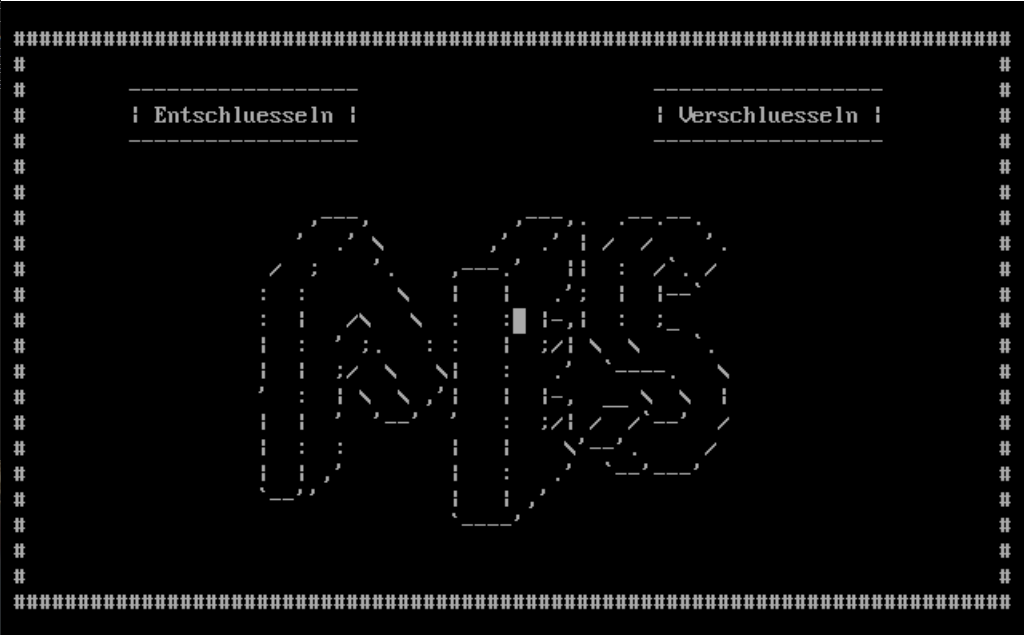
\includegraphics[width=0.72\textwidth]{images/tf1_hauptbildschirm.png}
    \caption{Hauptbildschirm -- der Cursor befindet sich in der Bildschirm-Mitte}
    \label{fig:tf1-haupt}
\end{figure}

\begin{figure}[H]
    \noindent\textbf{Maus über der Verschlüsselung:}\par\vspace{2mm}
    \centering
    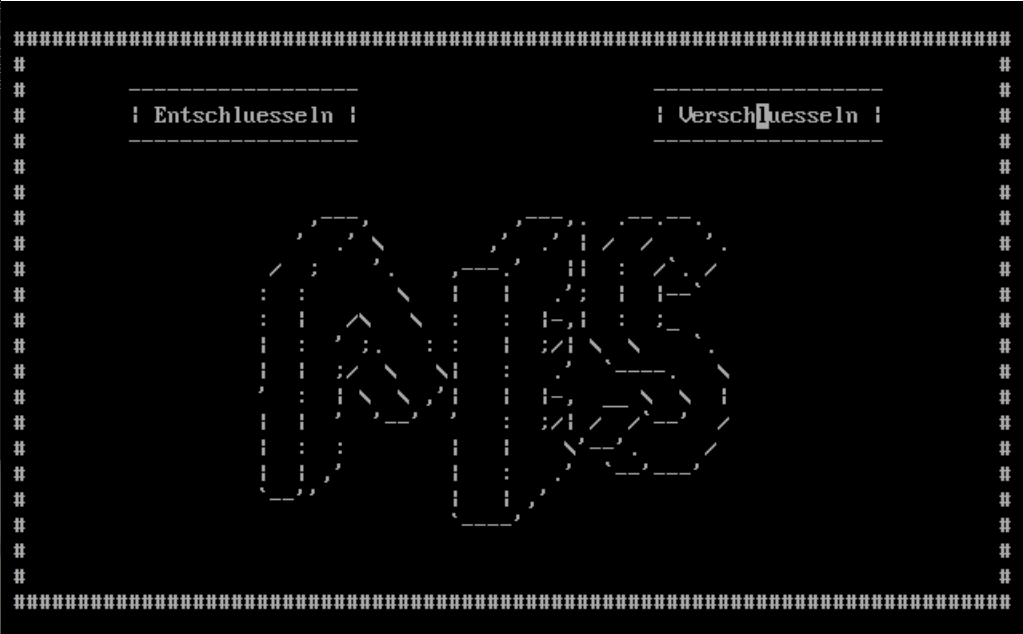
\includegraphics[width=0.72\textwidth]{images/tf1_maus_ueber_ver.png}
    \caption{Cursor über der Schaltfläche \glqq Verschluesseln\grqq}
    \label{fig:tf1-maus}
\end{figure}

\begin{figure}[H]
    \noindent\textbf{Nach dem Klick:}\par\vspace{2mm}
    \centering
    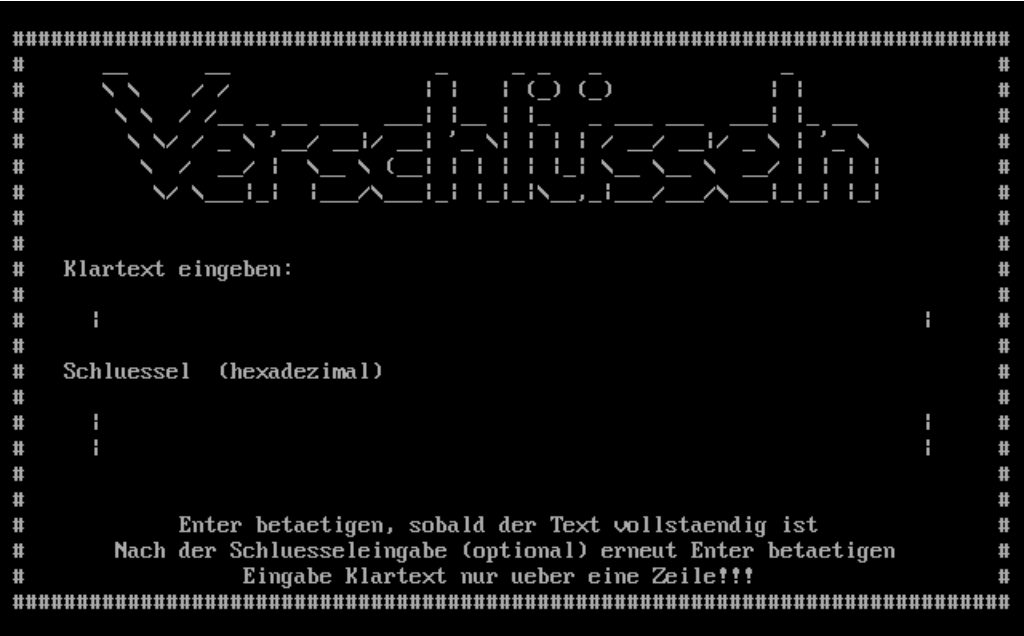
\includegraphics[width=0.72\textwidth]{images/tf1_nach_klick.png}
    \caption{Bildschirm nach dem Klick auf \glqq Verschluesseln\grqq}
    \label{fig:tf1-klick}
\end{figure}

%------------------------------------------------------------------------------
\Needspace{14\baselineskip}
\subsection{Testfall 2 -- SBOX-Substitution bei Ver- und Entschlüsseln}\label{sec:tf2}
\begin{figure}[H]
    \noindent\textbf{Eingabe Verschlüsselung}\par\vspace{2mm}
    \centering
    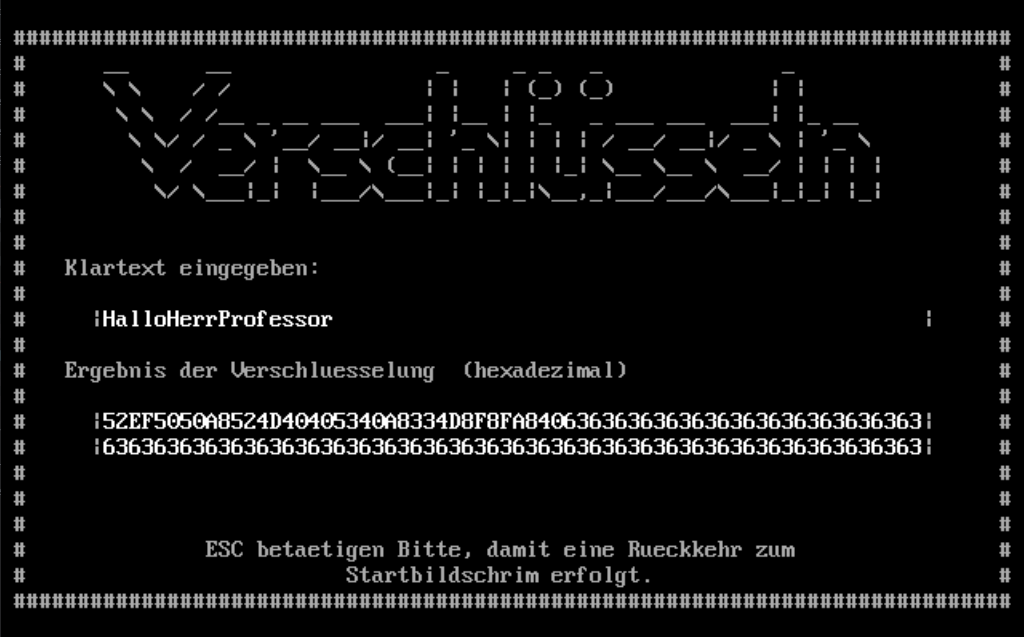
\includegraphics[width=0.72\textwidth]{images/tf2_ver_eingabe.png}
    \caption{Testfall 2: Eingabe \glqq HalloHerrProfessor\grqq{} und Ergebnis der Verschlüsselung}
    \label{fig:tf2-ver}
\end{figure}

\begin{table}[H]
    \noindent\textbf{Beweis:}\par\vspace{2mm}
    \centering
    \small
    \renewcommand{\arraystretch}{1.05}
    \caption{Testfall 2: SBOX-Substitution}\label{tab:tf2}
    \begin{tabular}{|l|l|l|c|}
        \hline
        \textbf{Buchstabe} & \textbf{HexWert (ASCII)} & \textbf{Substitutionswert} & \\ \hline
        \sbrow{H}{48}{72}{52}
        \sbrow{a}{61}{97}{EF}
        \sbrow{l}{6C}{108}{50}
        \sbrow{l}{6C}{108}{50}
        \sbrow{o}{6F}{111}{A8}
        \sbrow{H}{48}{72}{52}
        \sbrow{e}{65}{101}{4D}
        \sbrow{r}{72}{114}{40}
        \sbrow{r}{72}{114}{40}
        \sbrow{P}{50}{80}{53}
        \sbrow{r}{72}{114}{40}
        \sbrow{o}{6F}{111}{A8}
        \sbrow{f}{66}{102}{33}
        \sbrow{e}{65}{101}{4D}
        \sbrow{s}{73}{115}{8F}
        \sbrow{s}{73}{115}{8F}
        \sbrow{o}{6F}{111}{A8}
        \sbrow{r}{72}{114}{40}
        \glqq 0\grqq{} (Nicht die ASCII 0) & \hexs{00} & \hexs{63} & \iconok \\ \hline
    \end{tabular}
\end{table}

Die große Menge an \glqq 63\grqq{} nach der Nachricht erscheinen durch den Hintergrund, dass der \asm{TastaturBuffer} (das Array zum Zwischenspeichern) mit 0 initialisiert ist und somit alle nicht überschriebenen Werte eine 0 innehaben.

\begin{figure}[H]
    \noindent\textbf{Gegeneingabe Entschlüsseln}\par\vspace{2mm}
    \centering
    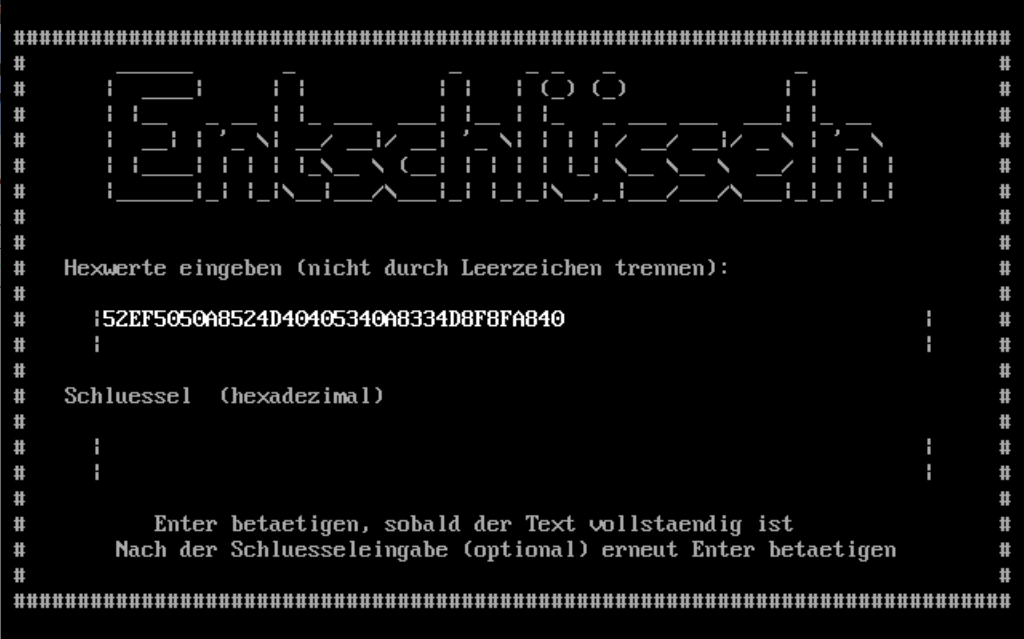
\includegraphics[width=0.72\textwidth]{images/tf2_ent_eingabe.png}
    \caption{Testfall 2: Eingabe des Chiffretextes zum Entschlüsseln}
    \label{fig:tf2-ent-ein}
\end{figure}

\begin{figure}[H]
    \centering
    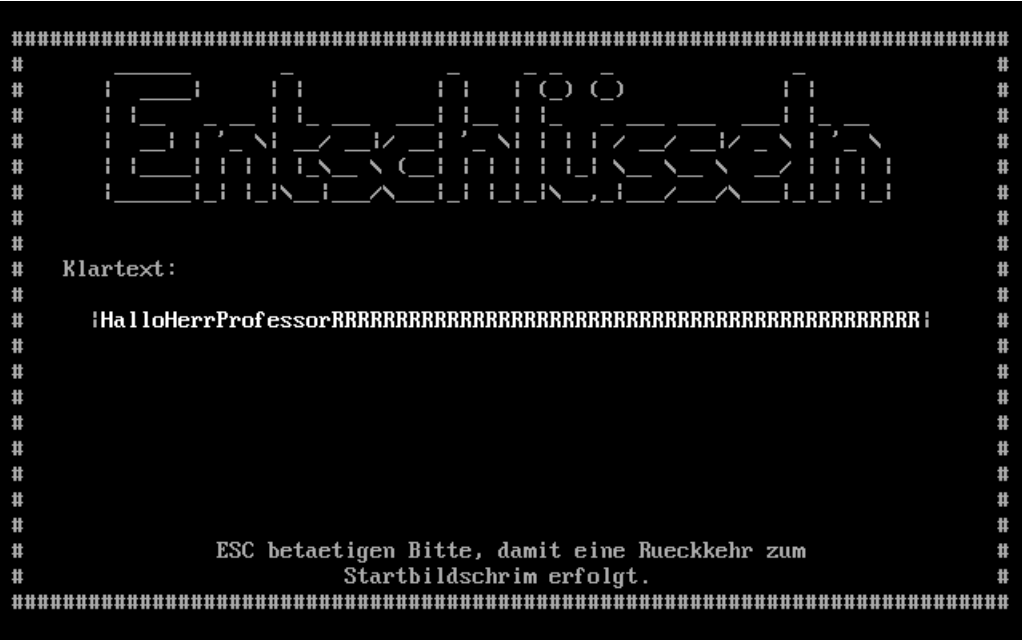
\includegraphics[width=0.72\textwidth]{images/tf2_ent_ergebnis.png}
    \caption{Testfall 2: Ergebnis der Entschlüsselung}
    \label{fig:tf2-ent-erg}
\end{figure}

Die ganzen \glqq R\grqq{} entstehen wieder durch die fehlende Eingabe (0 bei der invertierten SBox ist $52_{\text{hex}}$ und dies entspricht dem großen R).

%------------------------------------------------------------------------------
\Needspace{14\baselineskip}
\subsection{Testfall 3 -- ShiftRow \& Inverse}\label{sec:tf3}
\textbf{Stand 2.0.0:} Der Test war erfolgreich, deckte aber einen Fehler nicht auf: Der Text hat nur 18 Zeichen, der vierte Block (\asm{Pos 48}--\asm{63}) enthält nur Nullbytes, und deren Verschiebung ist unsichtbar. Tatsächlich wurde der vierte Block in 1.x nie verschoben (Abschnitt~\ref{sec:vers-shiftrow}). Seit 2.0.0 ist das behoben; ein Test mit 64 Zeichen steht in Teil~C aus.

\begin{figure}[H]
    \noindent\textbf{Eingabe Verschlüsselung}\par\vspace{2mm}
    \centering
    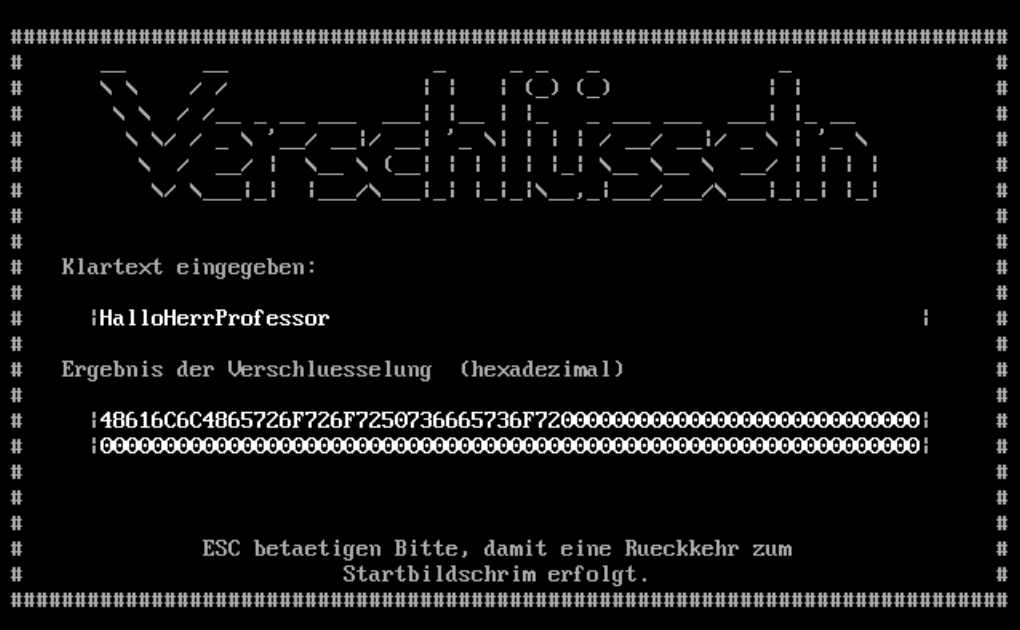
\includegraphics[width=0.72\textwidth]{images/tf3_ver_eingabe.png}
    \caption{Testfall 3: Eingabe \glqq HalloHerrProfessor\grqq{} und Ergebnis}
    \label{fig:tf3-ver}
\end{figure}

\begin{table}[H]
    \noindent\textbf{Beweis:}\par\vspace{2mm}
    \centering
    \small
    \renewcommand{\arraystretch}{1.05}
    \caption{Testfall 3: ShiftRow}\label{tab:tf3}
    \begin{tabular}{|l|l|l|c|}
        \hline
        \textbf{Buchstabe} & \textbf{HexWert (ASCII)} & \textbf{Verschoben} & \textbf{Blöcke} \\ \hline
        \srrow{H}{48}{72}{48}{72}{1}
        \srrow{a}{61}{97}{61}{97}{1}
        \srrow{l}{6C}{108}{6C}{108}{1}
        \srrow{l}{6C}{108}{6C}{108}{1}
        \srrow{o}{6F}{111}{48}{72}{2}
        \srrow{H}{48}{72}{65}{101}{2}
        \srrow{e}{65}{101}{72}{114}{2}
        \srrow{r}{72}{114}{6F}{111}{2}
        \srrow{r}{72}{114}{72}{114}{3}
        \srrow{P}{50}{80}{6F}{111}{3}
        \srrow{r}{72}{114}{72}{114}{3}
        \srrow{o}{6F}{111}{50}{80}{3}
        \srrow{f}{66}{102}{73}{115}{4}
        \srrow{e}{65}{101}{66}{102}{4}
        \srrow{s}{73}{115}{65}{101}{4}
        \srrow{s}{73}{115}{73}{115}{4}
        \srrow{o}{6F}{111}{6F}{111}{1}
        \srrow{r}{72}{114}{72}{114}{1}
        \glqq 0\grqq{} (Nicht die ASCII 0) & \hexs{00} & \hexs{00} & \cellcolor{blk1} 1 \\ \hline
    \end{tabular}
\end{table}

\begin{figure}[H]
    \noindent\textbf{Schema (Verschlüsselung ShiftRow):}\par\vspace{2mm}
    \centering
    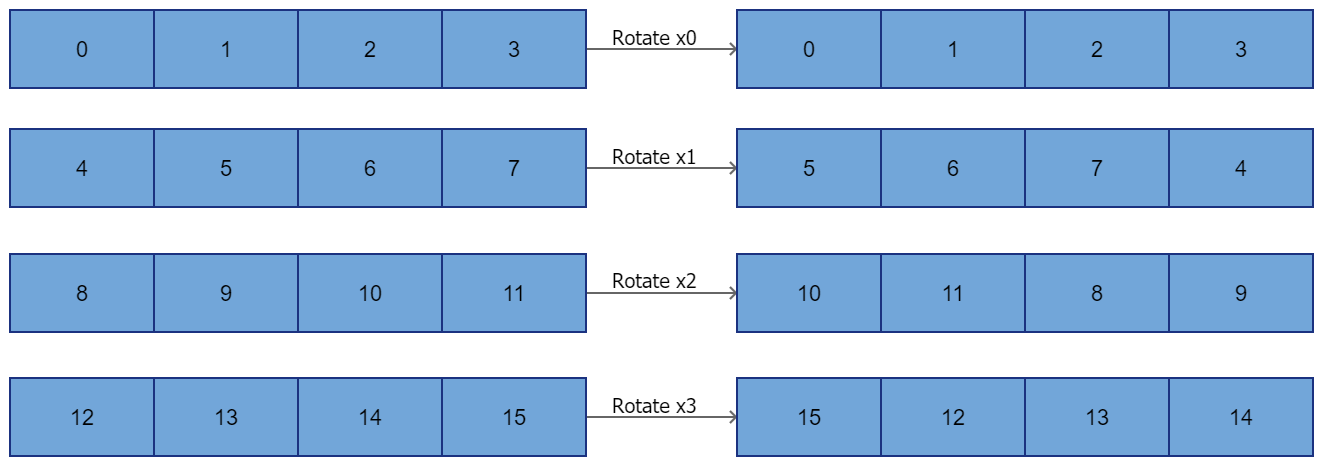
\includegraphics[width=\textwidth]{images/tf3_schema_shiftrow.png}
    \caption{Testfall 3: Schema der ShiftRow-Verschlüsselung}
    \label{fig:tf3-schema}
\end{figure}

\begin{figure}[H]
    \noindent\textbf{Gegeneingabe Entschlüsselung:}\par\vspace{2mm}
    \centering
    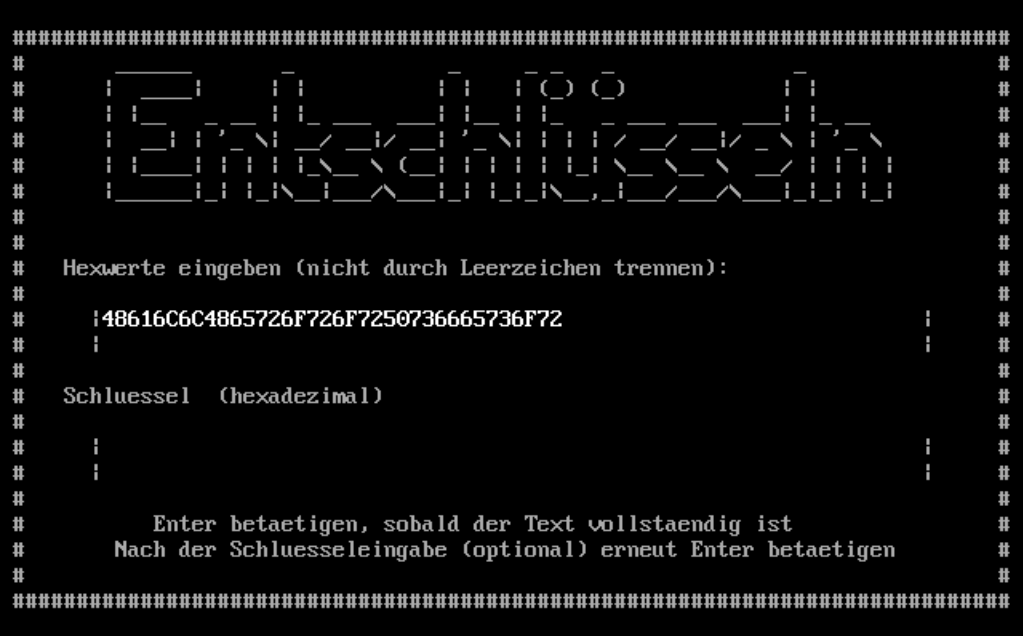
\includegraphics[width=0.72\textwidth]{images/tf3_ent_eingabe.png}
    \caption{Testfall 3: Eingabe des Chiffretextes zum Entschlüsseln}
    \label{fig:tf3-ent-ein}
\end{figure}

\begin{figure}[H]
    \centering
    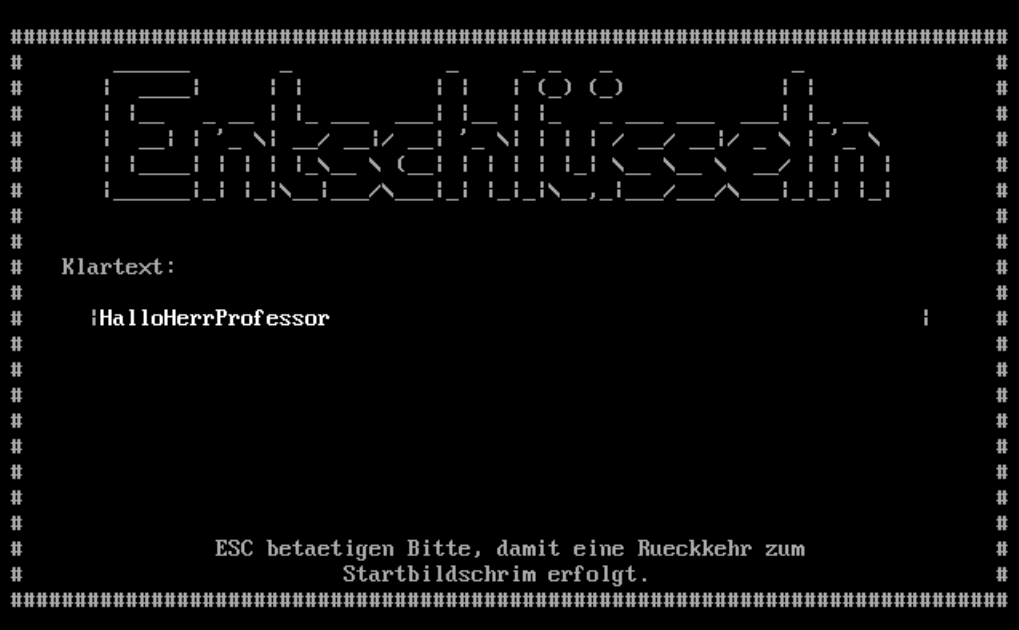
\includegraphics[width=0.72\textwidth]{images/tf3_ent_ergebnis.png}
    \caption{Testfall 3: Ergebnis der Entschlüsselung (ShiftRow invers)}
    \label{fig:tf3-ent-erg}
\end{figure}

%------------------------------------------------------------------------------
\Needspace{14\baselineskip}
\subsection{Testfall 4 -- ShiftColumn}\label{sec:tf4}
\textbf{Stand 2.0.0:} \asm{MalZweiPROC}, auf die \asm{ShiftColumn} aufbaut, wurde korrigiert (Abschnitt~\ref{sec:vers-shiftcolumn}). Die Prüfung gegen die Referenzvektoren steht in Abschnitt~\ref{sec:tests-modell} (M4, M6, M7). Wie damals wird \asm{ShiftColumn} nur in einem Einzeltest, nicht im aktiven Ablauf geprüft.

\begin{figure}[H]
    \centering
    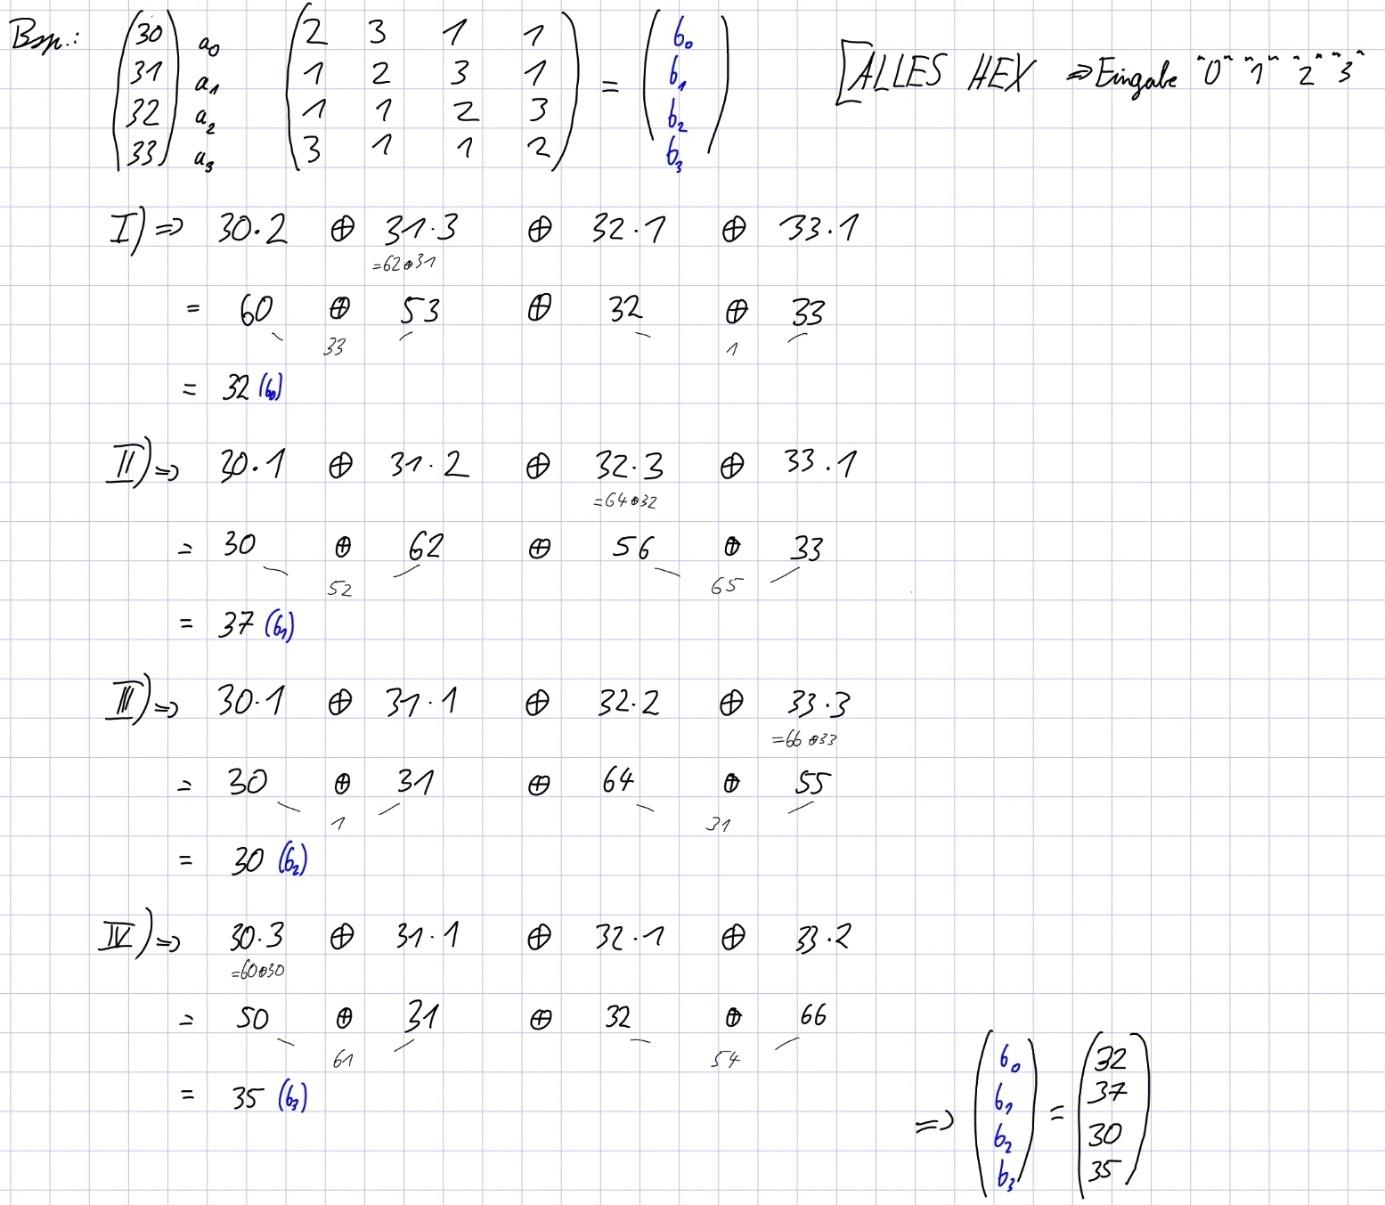
\includegraphics[width=0.95\textwidth]{images/tf4_handrechnung.png}
    \caption{Testfall 4: Handrechnung zur ShiftColumn}
    \label{fig:tf4-hand}
\end{figure}

\begin{figure}[H]
    \noindent\textbf{Screenshot:}\par\vspace{2mm}
    \centering
    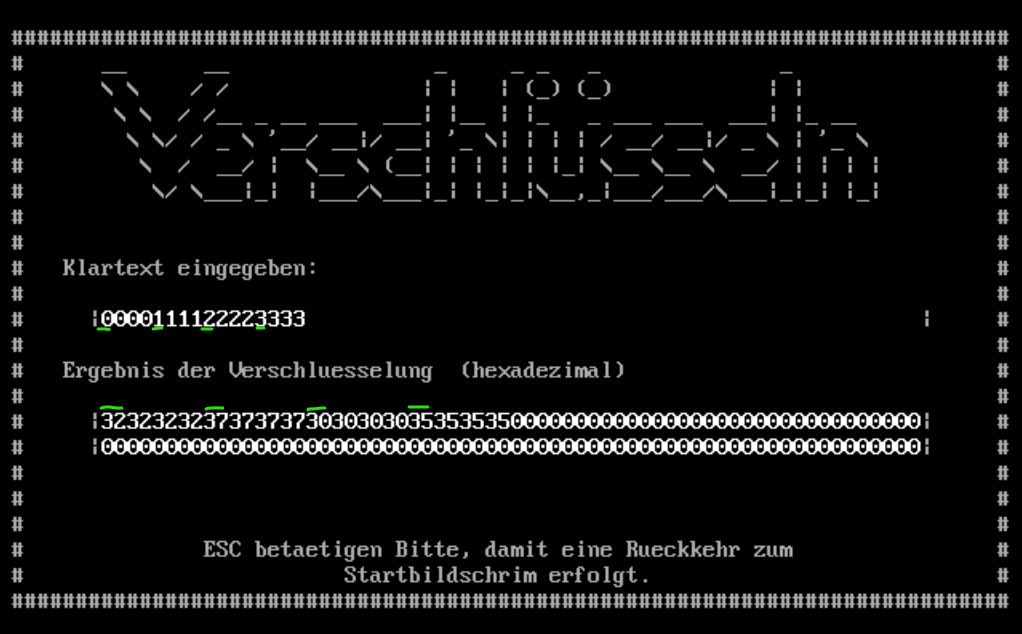
\includegraphics[width=0.72\textwidth]{images/tf4_screenshot.png}
    \caption{Testfall 4: Screenshot des Programmergebnisses}
    \label{fig:tf4-shot}
\end{figure}

%------------------------------------------------------------------------------
\Needspace{14\baselineskip}
\subsection{Testfall 5 -- ShiftColumn Invers}\label{sec:tf5}
Ergebnis in Version~1.x: fehlgeschlagen \iconfehler

\textbf{Stand 2.0.0:} Die PROC wurde neu geschrieben (Kapitel~\ref{sec:asm-dateien}, \asm{ShiftColumn_1}); die Handrechnung unten zeigt noch den damaligen Versuch. Das Ergebnis der neuen Fassung im Modell steht in M5 bis M7 (Abschnitt~\ref{sec:tests-modell}).

\begin{figure}[H]
    \centering
    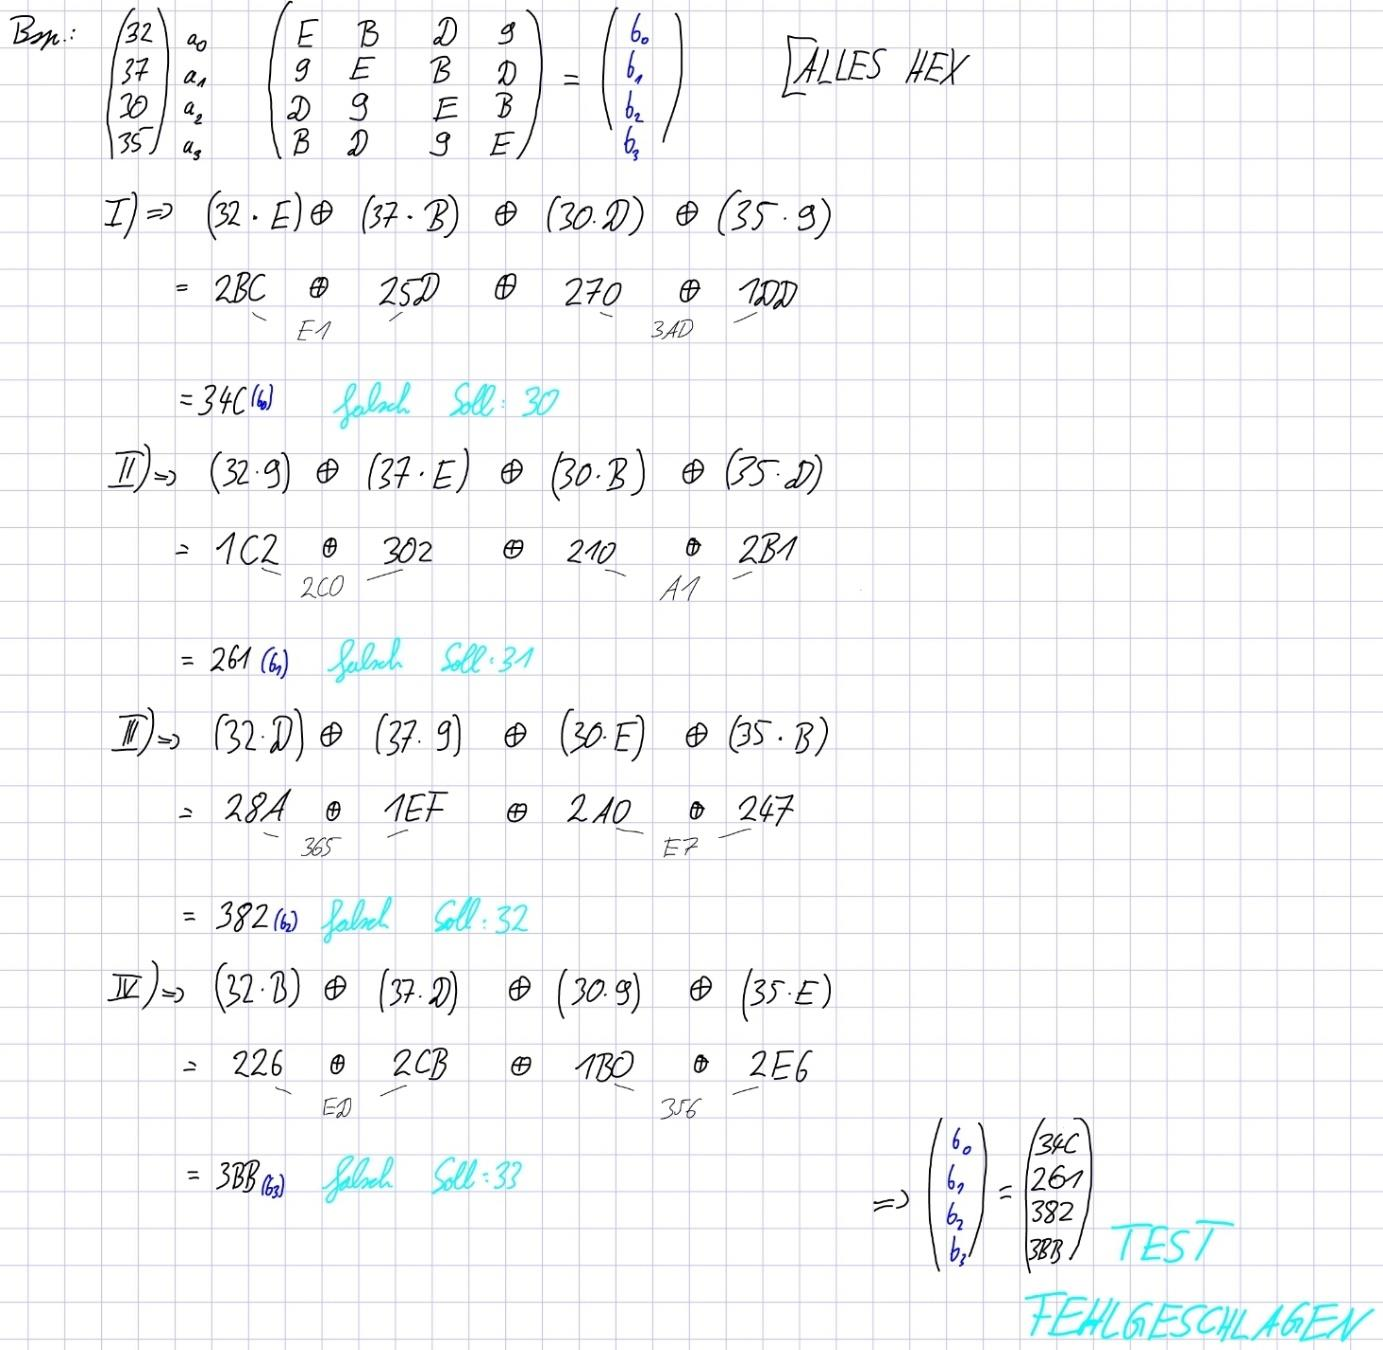
\includegraphics[width=0.95\textwidth]{images/tf5_handrechnung.png}
    \caption{Testfall 5: Handrechnung zur inversen ShiftColumn}
    \label{fig:tf5-hand}
\end{figure}

%------------------------------------------------------------------------------
\Needspace{14\baselineskip}
\subsection{Testfall 6 -- SchluesselAnwenden (PROC)}\label{sec:tf6}
Es wird hier der implementierte Standardschlüssel ohne Expansion verwendet zur Demonstration.

\begin{table}[H]
    \noindent\textbf{Theoretisch:}\par\vspace{2mm}
    \centering
    \small
    \renewcommand{\arraystretch}{1.05}
    \caption{Testfall 6: Anwenden des Standardschlüssels (XOR)}\label{tab:tf6}
    \begin{tabular}{|l|l|l|l|}
        \hline
        \textbf{Buchstabe} & \textbf{HexWert (ASCII)} & \textbf{Schlüsselwert} & \textbf{XOR Ergebnis} \\ \hline
        \sarow{H}{48}{72}{51}{19}
        \sarow{a}{61}{97}{DB}{BA}
        \sarow{l}{6C}{108}{AD}{C1}
        \sarow{l}{6C}{108}{CF}{A3}
        \sarow{o}{6F}{111}{83}{EC}
        \sarow{H}{48}{72}{9F}{D7}
        \sarow{e}{65}{101}{BD}{D8}
        \sarow{r}{72}{114}{27}{55}
        \sarow{r}{72}{114}{B7}{C5}
        \sarow{P}{50}{80}{FF}{AF}
        \sarow{r}{72}{114}{25}{57}
        \sarow{o}{6F}{111}{8A}{E5}
        \sarow{f}{66}{102}{1F}{79}
        \sarow{e}{65}{101}{A6}{C3}
        \sarow{s}{73}{115}{B3}{C0}
        \sarow{s}{73}{115}{91}{E2}
        \sarow{o}{6F}{111}{FB}{94}
        \sarow{r}{72}{114}{9C}{EE}
    \end{tabular}
\end{table}

\begin{figure}[H]
    \noindent\textbf{Screenshot als Beweis:}\par\vspace{2mm}
    \centering
    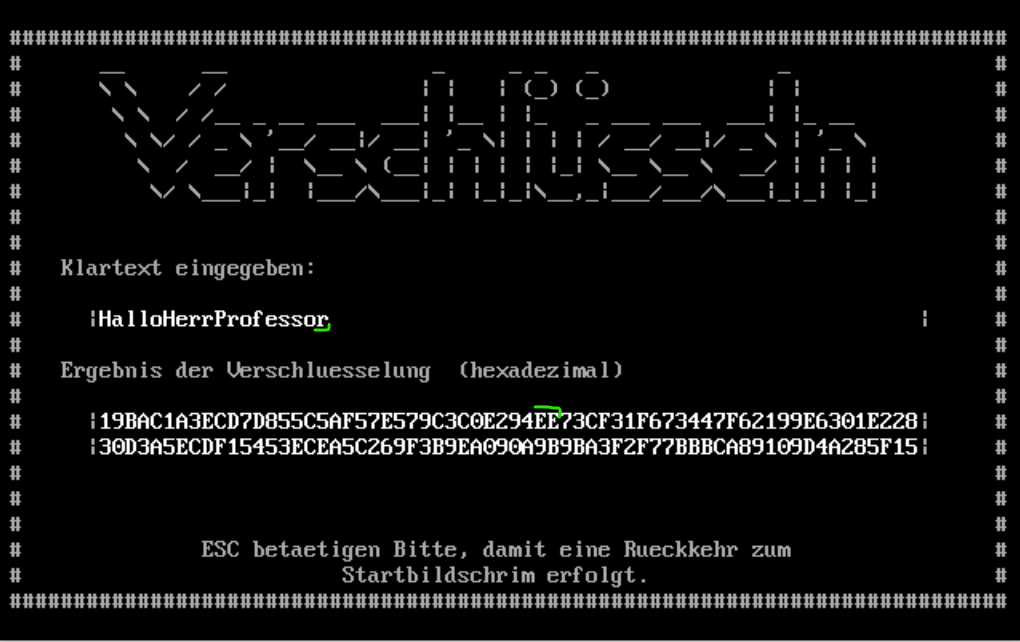
\includegraphics[width=0.72\textwidth]{images/tf6_screenshot.png}
    \caption{Testfall 6: Screenshot als Beweis}
    \label{fig:tf6-shot}
\end{figure}

%------------------------------------------------------------------------------
\Needspace{14\baselineskip}
\subsection{Modellprüfung der Version \versionProjekt}\label{sec:tests-modell}
Zu Version~\versionProjekt\ gehört das Skript \asm{Dokumentation/Modelltest/modelltest.py}. Es bildet die Prozeduren \asm{SchluesselInitialisieren}, \asm{SchluesselAnwenden}, \asm{Schluesselexpansion}, \asm{SBOXSubstitution}, \asm{ShiftRow}, \asm{MalZweiPROC}, \asm{GFMulPROC}, \asm{ShiftColumn} und ihre Gegenstücke Schritt für Schritt (gleiche Register- und Speicherbelegung, gleiche Schleifen) in Python nach und liest die Tabellen direkt aus \asm{SBOX.asm} und \asm{config.asm}. Geprüft wird gegen Referenzen, die nicht aus dem Assemblercode stammen: die AES-S-Box aus ihrer Definition, die Multiplikation in $\mathrm{GF}(2^8)$ per Polynomdivision, Testvektoren aus \cite{fips197} bzw.\ der MixColumns-Literatur und eine Formel für \asm{ShiftRow}.

\begin{table}[!htbp]
    \centering
    \small
    \renewcommand{\arraystretch}{1.1}
    \caption{Modellprüfung -- Ergebnisse von \texttt{modelltest.py}}\label{tab:tests-modell}
    \begin{tabular}{@{}lp{6.2cm}p{5.6cm}@{}}
        \toprule
        \textbf{Nr.} & \textbf{Prüfung} & \textbf{Umfang / Ergebnis} \\
        \midrule
        M1 & S-Box und inverse S-Box gleich der AES-S-Box \cite{fips197} & 256 Einträge je Tabelle \iconok \\
        M2 & \asm{ShiftRow} und \asm{ShiftRow_1}, alle vier Blöcke & 300 Zufallszustände, Block 4 einzeln \iconok \\
        M3 & Schlüsselexpansion & $K_1=$ \asm{65 BE 13 DC}\ldots, $K_2=$ \asm{7A C4 D7 0B}\ldots; Konstante \asm{5F}, \asm{BE}, \asm{7D} \iconok \\
        M4 & \asm{MalZweiPROC} & alle 256 Eingaben \iconok \\
        M5 & \asm{GFMulPROC} & alle 65\,536 Paare \iconok \\
        M6 & \asm{ShiftColumn} und \asm{ShiftColumn_1} gegen Testvektoren & 6 Vektoren (u.\,a. \asm{DB 13 53 45} $\to$ \asm{8E 4D A1 BC}), alle 16 Spalten \iconok \\
        M7 & \asm{ShiftColumn} und Umkehrung, zufällig & 2000 Zustände \iconok \\
        M8 & Verschlüsselung \glqq Hallo\grqq{} & Chiffrat wie in Kapitel~\ref{sec:ablauf-beispiel} \iconok \\
        M9 & Ver- und Entschlüsseln, Standardschlüssel & 500 Zufallstexte \iconok \\
        M10 & Ver- und Entschlüsseln, eigener (Teil-)Schlüssel & 500 Fälle \iconok \\
        M11 & vierter Block wird verarbeitet & \asm{Pos 48}--\asm{63} \iconok \\
        \bottomrule
    \end{tabular}
\end{table}

\textbf{Aussagekraft.} Die Modellprüfung belegt, dass die \emph{Logik} der Assemblerroutinen stimmt. Sie belegt nicht, dass der Quelltext fehlerfrei übersetzt wird, dass die Register im echten Lauf die angenommenen Werte haben (z.\,B.\ \asm{DS}/\asm{ES}) oder dass die Bildschirmausgabe stimmt. Dafür sind die DOS-Box-Tests in Abschnitt~\ref{sec:tests-dosbox} nötig. Beim Schreiben des Skripts fiel auf, dass die Tabelle \asm{s_1_0} einen Eintrag \asm{0D5H} (großes \asm{H}) enthält; Programme, die die Tabelle auswerten, müssen die Groß-/Kleinschreibung des Suffixes beachten (TASM akzeptiert beides).

%------------------------------------------------------------------------------
\Needspace{14\baselineskip}
\subsection{Noch auszuführen: Tests in der DOS-Box (Version \versionProjekt)}\label{sec:tests-dosbox}
Diese Tests sind für Version~\versionProjekt\ noch von Hand durchzuführen (\asm{asmaes.bat}, dann \asm{start.bat}). Die erwarteten Werte stammen aus dem Modell (Teil~B). Die Spalte \glqq Ergebnis\grqq{} ist absichtlich leer.

\begin{table}[!htbp]
    \centering
    \small
    \renewcommand{\arraystretch}{1.15}
    \caption{DOS-Box-Tests für Version \versionProjekt}\label{tab:tests-dosbox}
    \begin{tabular}{@{}lp{3.1cm}p{5.9cm}c@{}}
        \toprule
        \textbf{Nr.} & \textbf{Eingabe} & \textbf{Erwartung} & \textbf{Ergebnis} \\
        \midrule
        D1 & Programm kompilieren und starten & fehlerfrei übersetzt; Hauptbildschirm erscheint & \\
        D2 & Verschlüsseln: \texttt{Hallo}, \asm{Enter}, \asm{Enter} & Chiffrat \asm{E159BDA8 8E0FB958 ...}, vollständig Listing~\ref{lst:beispiel-chiffrat} & \\
        D3 & Entschlüsseln: Chiffrat aus D2, \asm{Enter}, \asm{Enter} & \texttt{Hallo}, dahinter Leerstellen & \\
        D4 & Verschlüsseln: \texttt{Hallo}, eigener Schlüssel \asm{01} $\times 64$ (128 Ziffern \texttt{01}) & beginnt mit \asm{E9B50FF0 A2378E6D}; Entschlüsseln mit demselben Schlüssel liefert \texttt{Hallo} & \\
        D5 & Verschlüsseln: \texttt{Hallo}, Teilschlüssel \texttt{5F} (nur ein Byte) & beginnt mit \asm{3E655D79 1E745EBC} & \\
        D6 & Verschlüsseln: 64 Zeichen, Text siehe unter der Tabelle & beginnt mit \asm{BF3DF6BD FC3592CE}, endet mit \asm{... 97D9733B}; Rückweg liefert den Text & \\
        D7 & Entschlüsseln mit falschem Schlüssel & kein \texttt{Hallo}, nur Zeichensalat & \\
        \bottomrule
    \end{tabular}
\end{table}

Der Text für D6 ist \texttt{ABCDEFGHIJKLMNOPQRSTUVWXYZ} gefolgt von \texttt{abcdefghijklmnopqrstuvwxyz} und \texttt{0123456789+-} (zusammen 64 Zeichen, ohne Leerzeichen).

D6 prüft insbesondere den vierten Block (\asm{Pos 48}--\asm{63}), der bei Version~1.0 nicht verschoben wurde. D4 und D5 prüfen die Schlüsseleingabe, die bis Version~1.0 wirkungslos war. Erst nach Abarbeitung dieser Tabelle ist Version~\versionProjekt\ im eigentlichen Sinn getestet.

                  % Test(s).pdf

    \nocite{*}
    \newpage
    \phantomsection
    \printbibheading[title={Quellen}]
    \addcontentsline{toc}{section}{Quellen}
    % \printbibliography[type=book, heading=subbibliography, title={Bücher}]  % keine Buecher vorhanden
    \printbibliography[type=online, heading=subbibliography, title={Links}]

    \newpage
    \phantomsection
    \listoffigures
    \addcontentsline{toc}{section}{\listfigurename}

    \newpage
    \phantomsection
    \addcontentsline{toc}{section}{\listtablename}
    \listoftables

    \newpage
    \phantomsection
    \addcontentsline{toc}{section}{\lstlistlistingname}
    \lstlistoflistings

    % Die Eidesstattliche Erklaerung beider Autoren steht in
    % section/funktionalitaet.tex (inkl. Unterschriften).

\end{document}
